% \documentclass[preprint,12pt,authoryear]
% {elsarticle}

\documentclass[12pt,authoryear]
{article}

\usepackage{authblk}
%----------------------------------------------------------------------
%% Basic math input
%----------------------------------------------------------------------
\usepackage{amsmath}
\usepackage{amssymb}
\usepackage{amsfonts}
\usepackage{cancel}
\usepackage{amsthm}
\usepackage{mathtools}
\usepackage{comment}
%\usepackage{braket}
\allowdisplaybreaks

%----------------------------------------------------------------------
%% Fonts and alphabets (beware of conflicts)
%----------------------------------------------------------------------
%\usepackage[utf8]{inputenc}
%\usepackage{palatino}
\usepackage[T1]{fontenc}
\usepackage[mathscr]{eucal}
%\usepackage{dsfont} 
%\usepackage{calrsfs}
\usepackage{dsfont}


%----------------------------------------------------------------------
%% Document layout
%----------------------------------------------------------------------
%\setlength{\textwidth}{\paperwidth}
%\addtolength{\textwidth}{-2in}
%\calclayout
\usepackage{fullpage}
\newcommand{\afterhead}{.}
%\usepackage{titlesec}
%
%\newcommand{\afterhead}[1]{#1.}
%
%\titleformat{\section}[runin]{\bfseries}{\thesection.}{1ex}{\afterhead}
%\titlespacing{\section}{1em}{1.25em}{1em}
\usepackage{setspace}



%----------------------------------------------------------------------
%% Miscellaneous
%----------------------------------------------------------------------
\usepackage{acronym}
\usepackage{enumitem}
\usepackage{latexsym}
\usepackage{longtable}
%\usepackage{paralist}
\usepackage{wasysym}
\usepackage{xspace}

%----------------------------------------------------------------------
%% Colors
%----------------------------------------------------------------------
\usepackage[dvipsnames,svgnames]{xcolor}
\colorlet{MyBlue}{DodgerBlue!60!Black}
\colorlet{MyGreen}{DarkGreen!85!Black}


%----------------------------------------------------------------------
%% Figures and Graphics
%----------------------------------------------------------------------
\usepackage[font=small,labelfont=bf]{caption}
%\captionsetup[algorithm]{labelfont={bf,sf,normalsize},font={small},labelsep=period}
\usepackage{subfigure}
\usepackage{tikz}
\usetikzlibrary{positioning, arrows.meta}
\usetikzlibrary{calc,patterns}


%----------------------------------------------------------------------
%% References
%----------------------------------------------------------------------
\usepackage[authoryear,comma]{natbib}
\def\bibfont{\footnotesize}
\def\bibsep{2pt}
\def\bibhang{24pt}
\def\BIBand{and}
\def\newblock{\ }
%\bibpunct[, ]{[}{]}{,}_{n}{}{,}

\newcommand{\citeor}[2][]{\citeauthor{#2} \cite[#1]{#2}}
\newcommand{\citeorp}[2][]{\textup(\citeor[#1]{#2}\textup)}



%----------------------------------------------------------------------
%% Hyperlinks
%----------------------------------------------------------------------
\usepackage{hyperref}
\hypersetup{
colorlinks=true,
linktocpage=true,
%pdfstartpage=1,
pdfstartview=FitH,
breaklinks=true,
pdfpagemode=UseNone,
pageanchor=true,
pdfpagemode=UseOutlines,
plainpages=false,
bookmarksnumbered,
bookmarksopen=false,
bookmarksopenlevel=1,
hypertexnames=true,
pdfhighlight=/O,
%hyperfootnotes=true,
%nesting=true,
%frenchlinks,
urlcolor=MyBlue!60!black,
linkcolor=MyBlue!70!black,
citecolor=DarkGreen!70!black, % <--- for screen
%urlcolor=black, linkcolor=black, citecolor=black, %pagecolor=black, % <--- for printing
%pagecolor=RoyalBlue,
pdftitle={},
pdfauthor={},
pdfsubject={},
pdfkeywords={},
pdfcreator={pdfLaTeX},
pdfproducer={LaTeX with hyperref}
}

% Hyperlink shortcuts
%\renewcommand{\EMAIL}[1]{\href{mailto:#1}{\texttt{#1}}}
%\def\URL#1{\href{#1}{#1}}




%----------------------------------------------------------------------
%% Cleverefs
%----------------------------------------------------------------------
\numberwithin{equation}{section}  %numberwithin goes before cleverefs when using hyperref
\usepackage[sort&compress,capitalize,nameinlink]{cleveref}
%\crefname{example}{Ex.}{Exs.}
\crefname{app}{Appendix}{Appendices}
\newcommand{\crefrangeconjunction}{\textendash}
\crefrangeformat{equation}{\upshape(#3#1#4)\textendash(#5#2#6)}


%*************************************************************
%*****    EDITING
%*************************************************************
\usepackage[textwidth=30mm]{todonotes}

%\setlength{\marginparwidth}{2cm}
\usepackage{soul}
\setstcolor{red}
\sethlcolor{SkyBlue}

\newcommand{\needref}{{\color{red} \upshape [\textbf{??}]}\xspace}
\newcommand{\attn}{{\color{red} \upshape [\textbf{!!}]}\xspace}
\newcommand{\revise}[1]{{\color{blue}#1}}
\newcommand{\lookout}[1]{{\bfseries\color{red}[#1]}}
\newcommand{\hilite}[1]{#1}
%\newcommand{\debug}[1]{{\color{purple}#1}}
\newcommand{\debug}[1]{#1}



%*************************************************************
%*****    ENVIRONMENTS
%*************************************************************

%----------------------------------------------------------------------
%% Algorithms
%----------------------------------------------------------------------
%\usepackage{algorithm2e_extension}
%\usepackage{algorithm2e}
%\usepackage{algorithm}
%\SetKwBlock{Repeat}{Repeat}{}
%\SetKwProg{SimulForEach}{for each}{\;do simultaneously}{}
%\newcommand{\kwd}[1]{\textsf{\bfseries#1}}
\usepackage[linesnumbered,ruled,vlined]{algorithm2e}
\newcommand\mycommfont[1]{\scriptsize\ttfamily\textcolor{gray}{#1}}
\SetCommentSty{mycommfont} % Edit the font + style of comments in algorithm
\SetAlgoSkip{bigskip} % adjust space before algorithm


%----------------------------------------------------------------------
%% Theorem-like
%----------------------------------------------------------------------
\theoremstyle{plain}
\newtheorem{theorem}{Theorem}
\newtheorem{corollary}[theorem]{Corollary}
% \newtheorem*{corollary*}{Corollary}
\newtheorem{lemma}[theorem]{Lemma}
\newtheorem{proposition}[theorem]{Proposition}
\newtheorem{conjecture}[theorem]{Conjecture}
\newtheorem{claim}[theorem]{Claim}

%----------------------------------------------------------------------
%% Definition-like
%----------------------------------------------------------------------
\theoremstyle{definition}
\newtheorem{definition}[theorem]{Definition}
% \newtheorem*{definition*}{Definition}
\newtheorem{assumption}[theorem]{Assumption}
\newtheorem{hypothesis}{Hypothesis}
% \newtheorem*{hypothesis*}{Hypothesis}
\newtheorem{notation}{Notation}


%----------------------------------------------------------------------
%% Remark-like
%----------------------------------------------------------------------
\theoremstyle{remark}
\newtheorem{remark}[theorem]{Remark}
% \newtheorem*{remark*}{Remark}
% \newtheorem*{notation*}{Notational remark}
\newtheorem{example}[theorem]{Example}


%----------------------------------------------------------------------
%% Proofs
%----------------------------------------------------------------------
%\newenvironment{Proof}[1][Proof]{\begin{proof}[#1]}{\end{proof}}
%\renewcommand\qedsymbol{\small$\blacksquare$}


%----------------------------------------------------------------------
%% Numbering
%----------------------------------------------------------------------
\numberwithin{theorem}{section}
%\numberwithin{remark}{section}
%\numberwithin{example}{section}



%*************************************************************
%*****    FREQUENTLY USED
%*************************************************************


%----------------------------------------------------------------------
%% Delimiters
%----------------------------------------------------------------------
\providecommand\given{} % provides an empty command for the delimiters below

\DeclarePairedDelimiter{\braces}{\{}{\}}
\DeclarePairedDelimiter{\bracks}{[}{]}
\DeclarePairedDelimiter{\parens}{(}{)}

\DeclarePairedDelimiter{\abs}{\lvert}{\rvert}
\DeclarePairedDelimiter{\infloor}{\lfloor}{\rfloor}
\DeclarePairedDelimiter{\norm}{\lVert}{\rVert}
%\DeclarePairedDelimiter{\dnorm}{\lVert}{\rVert_{\ast}}
\newcommand{\dnorm}[1]{\norm{#1}_{\ast}}

\DeclarePairedDelimiter{\ceil}{\lceil}{\rceil}
\DeclarePairedDelimiter{\floor}{\lfloor}{\rfloor}
\DeclarePairedDelimiter{\clip}{[}{]}
\DeclarePairedDelimiter{\negpart}{[}{]_{-}}
\DeclarePairedDelimiter{\pospart}{[}{]_{+}}

\DeclarePairedDelimiter{\bra}{\langle}{\rvert}
\DeclarePairedDelimiter{\ket}{\lvert}{\rangle}
%\DeclarePairedDelimiterX{\braket}[2]{\langle}{\rangle}{#1\mathopen{}\hspace{1pt}\delimsize\vert\hspace{1pt}\mathopen{}#2}
\DeclarePairedDelimiterX{\braket}[2]{\langle}{\rangle}{#1,#2}

\DeclarePairedDelimiterX{\inner}[2]{\langle}{\rangle}{#1,#2}
\DeclarePairedDelimiterX{\setdef}[2]{\{}{\}}{#1:#2}

\DeclarePairedDelimiterXPP{\probof}[1]{\Prob}{(}{)}{}{%
\renewcommand\given{\nonscript\,\delimsize\vert\nonscript\,\mathopen{}}
#1}

\DeclarePairedDelimiterXPP{\exof}[1]{\Expect}{[}{]}{}{%
\renewcommand\given{\nonscript\,\delimsize\vert\nonscript\,\mathopen{}}
#1}



%----------------------------------------------------------------------
%% Math
%----------------------------------------------------------------------
\DeclareMathOperator{\adj}{\debug {adj}}
\DeclareMathOperator{\card}{\debug {card}}
\DeclareMathOperator{\expo}{\debug {e}}
\DeclareMathOperator{\trace}{\debug {tr}}

\newcommand{\diff}{\ \textup{\debug d}}

\newcommand{\naturals}{\mathbb{\debug N}}
\newcommand{\reals}{\mathbb{\debug R}}
\newcommand{\ident}{\debug I}
\newcommand{\ortho}{\debug U}
\newcommand{\jordan}{\debug J}
\newcommand{\genmatr}{\debug M}
\newcommand{\simplex}{\debug \Sigma}
\newcommand{\run}{\debug n}
\newcommand{\h}{\boldsymbol{h}}
\newcommand{\w}{\boldsymbol{w}}
\newcommand{\x}{\boldsymbol{x}}
\newcommand{\y}{\boldsymbol{y}}

%----------------------------------------------------------------------
%% Probability
%----------------------------------------------------------------------

\newcommand{\Prw}{\mathsf{\debug W}}
\newcommand{\mW}{\mathsf{\debug{\widetilde{W}}}}
\newcommand{\initial}{\debug \mu}
\newcommand{\transit}{\debug \pi}
\newcommand{\transitvec}{\boldsymbol{\transit}}
\newcommand{\transitvecalt}{\transitvec'}
\newcommand{\transitmatrix}{\debug \Pi}
\newcommand{\transitmatrixalt}{\transitmatrix'}
\newcommand{\transits}{\debug {\mathcal{T}}}
\newcommand{\stationary}{\debug \rho}
\newcommand{\laplace}{\debug L}
\newcommand{\eigen}{\debug \lambda}
\newcommand{\limittransitmatrix}{\overline{\debug \Pi}}
\newcommand{\proba}{\debug p}
\newcommand{\distr}{\debug F}

\newcommand{\distrtau}{\debug H}
\newcommand{\intdist}{\debug \Phi}
\newcommand{\exptau}{\debug \mu}

\DeclareMathOperator{\Expect}{\debug{\mathsf{E}}}
\DeclareMathOperator{\Prob}{\debug{\mathsf{P}}}
\DeclareMathOperator{\Gammad}{\mathsf{\debug{Gamma}}}
\DeclareMathOperator{\Beta}{\mathsf{\debug{Beta}}}
\DeclareMathOperator{\Binomial}{\mathsf{\debug{Binomial}}}
\DeclareMathOperator{\Exp}{\mathsf{\debug{Exp}}}
\DeclareMathOperator{\Geom}{\mathsf{\debug{Geom}}}
\DeclareMathOperator{\lr}{\debug{lr}}
\DeclareMathOperator{\Poisson}{\mathsf{\debug{Poisson}}}
\DeclareMathOperator{\stoch}{\debug{st}}
\DeclareMathOperator{\supp}{\debug{supp}}
\DeclareMathOperator{\Unif}{\mathsf{\debug{Unif}}}
\DeclareMathOperator{\Var}{\mathsf{\debug{Var}}}


%----------------------------------------------------------------------
%% Time
%----------------------------------------------------------------------
\newcommand{\horizon}{\debug T}




%----------------------------------------------------------------------
%% Network
%----------------------------------------------------------------------


%----------------------------------------------------------------------
%% Games
%----------------------------------------------------------------------
\newcommand{\game}{\debug \Gamma}

\newcommand{\play}{\debug i}
\newcommand{\playalt}{\debug j}
\newcommand{\nplayers}{\debug n}
%\newcommand{\players}{\mathcal{\nPlayers}}
\newcommand{\players}{\bracks{\nplayers}}
\newcommand{\pA}{\mathrm{\debug{A}}}
\newcommand{\pB}{\mathrm{\debug{B}}}


\newcommand{\pure}{\alpha}
\newcommand{\purealt}{\beta}
\newcommand{\nPures}{\debug S}
\newcommand{\pures}{\mathcal{\nPures}}
\newcommand{\peq}{\pure^{\ast}}

\newcommand{\actA}{\debug a}
\newcommand{\actAalt}{\actA'}
\newcommand{\actAaltalt}{\actA''}
\newcommand{\actB}{\debug b}
\newcommand{\actBalt}{\actB'}
\newcommand{\actBaltalt}{\actB''}
\newcommand{\actprof}{\boldsymbol{\act}}
\newcommand{\actprofalt}{\actprof'}
\newcommand{\acts}{\actions}
\newcommand{\intacts}{\intfeas}
\newcommand{\unactions}{\debug {\widetilde{\actions}}}
\newcommand{\nactions}{\debug K}
\newcommand{\nactionsstar}{\nactions^{\ast}}
\newcommand{\nactionsn}{\nactions_{\run}}
\newcommand{\nactionsA}{\nactions^{\pA}}
\newcommand{\nactionsB}{\nactions^{\pB}}
\newcommand{\nactionsAn}{\nactionsn^{\pA}}
\newcommand{\nactionsBn}{\nactionsn^{\pB}}
\newcommand{\actions}{[\nactions]}
\newcommand{\actionsA}{[\nactionsA]}
\newcommand{\actionsB}{[\nactionsB]}
\newcommand{\actionsAn}{[\nactionsAn]}
\newcommand{\actionsBn}{[\nactionsBn]}

\newcommand{\mixed}{\sigma}
\newcommand{\mixedprof}{\boldsymbol{\mixed}}


\newcommand{\cost}{\debug c}
\newcommand{\costprof}{\boldsymbol{\cost}}
\newcommand{\Cost}{\debug C}
\newcommand{\Costtype}{\debug \Cost_{\type}}
\newcommand{\CostA}{\debug \Cost_{\typeA}}
\newcommand{\CostB}{\debug \Cost_{\typeB}}
\newcommand{\costs}{\debug {\mathcal{C}}}

\newcommand{\pay}{\debug u}
\newcommand{\Pay}{\debug U}
\newcommand{\Bimatrix}{\boldsymbol{\Pay}}
\newcommand{\PayA}{\Pay^{\pA}}
\newcommand{\PayB}{\Pay^{\pB}}


\newcommand{\payv}{v}
\newcommand{\loss}{\ell}

\DeclareMathOperator{\brep}{BR}
\newcommand{\reg}{R}

\newcommand{\equilibria}{\mathcal{E}}

\newcommand{\cor}[1]{#1^{\ast}}
\newcommand{\eq}[1]{#1^{\ast}}
\newcommand{\optt}[1]{\tilde#1}
\newcommand{\out}[1]{\tilde#1}

\newcommand{\potential}{\debug \Psi}
\newcommand{\nequi}{\debug W}




\DeclareMathOperator{\BRD}{\mathsf{\debug{BRD}}}
\DeclareMathOperator{\cyclet}{\mathsf{\debug{cycle}}}
\DeclareMathOperator{\NE}{\mathsf{\debug{NE}}}












%---------------------------------------------------------------------
%% Sundries
%----------------------------------------------------------------------
\newcommand{\argdot}{\,\cdot\,}
\newcommand{\bigoh}{\mathcal{\debug{O}}}
\newcommand{\dkl}{D_{\textup{KL}}}
\newcommand{\filter}{\mathcal{F}}
\newcommand{\gen}{\mathcal{L}}
\newcommand{\ind}{\mathds{\debug 1}}
\newcommand{\interval}{\debug I}
%\newcommand{\simplex}{\Delta}
\newcommand{\intsimplex}{\simplex^{\!\circ}}
\newcommand{\set}{\mathcal{S}}
\newcommand{\smalloh}{\debug o}
\newcommand{\step}{\gamma}
\newcommand{\temp}{\eta}
 
\newcommand{\ie}{i.e., }
\newcommand{\eg}{e.g., }
\newcommand{\iid}{i.i.d.\ }
\newcommand{\rhs}{r.h.s.\ }
\newcommand{\lhs}{l.h.s.\ }

\DeclareMathOperator*{\argmax}{arg\,max}
\DeclareMathOperator*{\argmin}{arg\,min} 

%----------------------------------------------------------------------
% This paper
%----------------------------------------------------------------------
\newcommand{\arrtime}{\debug T}

\newcommand{\countN}{\debug N}

\newcommand{\exphit}{\debug h}

\newcommand{\benefit}{\debug \varphi} %Expected benefit
\newcommand{\benefitcust}{\benefit_{\cust}} %Expected benefit for player i
\newcommand{\benefitA}{\benefit_{\typeA}} %Expected benefit for player A
\newcommand{\benefitB}{\benefit_{\typeB}} %Expected benefit for player B
\newcommand{\benefitn}{\debug \psi} 
\newcommand{\benefitnB}{\benefitn_{\typeB}} %Expected benefit for player B
\newcommand{\cust}{\debug i}
\newcommand{\Etime}{\debug E} %Expected time of arrival at service
\newcommand{\Htime}{\debug H} %Expected time of RW in rectangle
\newcommand{\Exittime}{\widehat{\debug E}} % Expected exit time from the triangle 
\newcommand{\Preward}{\debug P}%probability to finish the service before  reneging
\newcommand{\hittingt}{\debug H}
\newcommand{\hittingtpr}{\debug{\widetilde{\hittingt}}}
\newcommand{\hitzero}{\debug \eta}
\newcommand{\hitzeroren}{\debug \kappa}

\newcommand{\statei}{\debug i}
\newcommand{\statej}{\debug j}

\newcommand{\meq}{ \widehat{\debug M}_{\equ}} %threshold no-preemp SS
\newcommand{\Meq}{ \debug M_{\typeB}^{\equ}}%threshold preemp SS

\newcommand{\nA}{\nAB_{\typeA}} %number of customers A in queue
\newcommand{\nB}{\nAB_{\typeB}} %number of customers A in queue
\newcommand{\nAB}{\debug n}% n=\nA+\nB
\newcommand{\NA}{\debug N_{\typeA}} %RV number of customer A
\newcommand{\NB}{\debug N_{\typeB}} %RV number of customer B
\newcommand{\optn}{\nAB^{\opt}}

\newcommand{\nunsol}{\nAB^{*}}
\newcommand{\NAB}{\widehat{\debug J}_{\typeA}}

\newcommand{\naor}{\debug M_{\typeA}} %Naor threshold 
\newcommand{\ncust}{\debug X} % number of customers in the queue (Markov chain)
\newcommand{\ncustY}{\debug Y} % number of customers in the queue (birth & death process)

\newcommand{\eqn}{\nAB^{\expo}}

\newcommand{\rate}{\debug \lambda} % generic rate
\newcommand{\rateA}{\debug \rate_{\typeA}} % arrival rate of customers A
\newcommand{\rateB}{\debug \rate_{\typeB}} %% arrival rate of customers B
\newcommand{\rateS}{\debug \mu} % Service rate of the server
\newcommand{\ratetype}{\debug \rate_{\type}} %% arrival rate of customers theta
\newcommand{\reward}{\debug R} %Reward R
\newcommand{\rewardi}{\debug \reward_i} %Reward R_i
\newcommand{\rewardA}{\debug \reward_{\typeA}} %Reward R_A
\newcommand{\rewardB}{\debug \reward_{\typeB}} %Reward R_B
\newcommand{\rewardtype}{\reward_{\type}}
\newcommand{\rhsBjoins}{\debug \gamma}
\newcommand{\rtime}{\debug \tau} % stopping time
\newcommand{\round}{\debug k} %discrete time

\newcommand{\served}{\debug \sigma} %type of the customer who is being served
\newcommand{\servtime}{\debug S}

\newcommand{\state}{\debug \omega}

\newcommand{\ttime}{\debug t} % physical time
\newcommand{\type}{\debug \theta} %type
\newcommand{\typeA}{\debug A} %customer type A
\newcommand{\typeB}{\debug B} %customer type B
\newcommand{\utilization}{\debug \rho}
\newcommand{\utilizationA}{\debug \rho_{\typeA}} %utilization factor for type A
\newcommand{\utilizationtype}{\debug \rho_{\type}} %utilization factor for type theta
\newcommand{\Utime}{\debug U} 

\newcommand{\Veq}{ \debug V_{\typeB}} %threshold preemp FS
\newcommand{\Teq}{ \debug T_{\typeB}} %total threshold for B customers



\newcommand{\AClassOpt}{n^*_{\typeA}} %threshold mediator of class A
\newcommand{\BClassOpt}{n^*_{\typeB}} %threshold mediator of class B
\newcommand{\Opt}{n^*_{\typeB}} %threshold global mediator 
\newcommand{\optA}{\debug M^{*}_{\typeA}}
\newcommand{\Wtime}{\debug W} 

\DeclareMathOperator{\equ}{\debug{eq}}
\DeclareMathOperator{\opt}{\debug{opt}}

%----------------------------------------------------------------------
% Authors comments
%----------------------------------------------------------------------
\newcommand{\MD}[1]{\todo[color=red!10!gray!30,author=\textbf{Maurizio},inline]{\small #1\\}}
\newcommand{\MS}[1]{\todo[color=blue!10!red!30,author=\textbf{Marco},inline]{\small #1\\}}


  
%----------------------------------------------------------------------
%%% ACRONYMS
%----------------------------------------------------------------------
\newcommand{\acdef}[1]{\textit{\acl{#1}} \textpar{\acs{#1}}\acused{#1}}
\newcommand{\acdefp}[1]{\alert{\aclp{#1}} \textpar{\acsp{#1}}\acused{#1}}

\newacro{FCFS}{first-come first-served}
\newacro{LCFS}{last-come fist-served}

\newacro{BRD}{best response dynamics}
\newacro{NE}{Nash equilibrium}
\newacroplural{NE}[NE]{Nash equilibria}
\newacro{PNE}{pure Nash equilibrium}
\newacroplural{PNE}[PNE]{pure Nash equilibria}
\newacro{MNE}{mixed Nash equilibrium}
\newacroplural{MNE}[MNE]{mixed Nash equilibria}
\newacro{PFNE}{prior-free Nash equilibrium}
\newacroplural{PFNE}[PFNE]{prior-free Nash equilibria}
\newacro{KKT}{Karush\textendash Kuhn\textendash Tucker}
\newacro{FIP}{finite improvement property}
\newacro{CLT}{central limit theorem}

\newacro{iid}[i.i.d.]{independent and identically distributed}



\begin{document}




\title{Strategic Queues with Priority Classes}



\author{Maurizio D'Andrea}
\author{Marco Scarsini}

\affil{Dipartimento di Economia e Finanza, Luiss University,
Viale Romania 32,
00197 
Roma,
Italy}

\maketitle


\begin{abstract}

We consider a strategic M/M/1 queueing model under a \acl{FCFS} regime, where customers are split into two classes and class $\typeA$ has priority over class $\typeB$. 
Customers can decide whether to join the queue or balk, and, in case they have joined the queue, whether and when to renege.
We study the equilibrium strategies and compare the equilibrium outcome and the social optimum in the two cases where the social optimum is or is not constrained by priority.



\noindent
\textbf{Keywords:}
M/M/1, \acl{FCFS}, Markov perfect equilibrium, social optimum, priority classes.




%\MSC[2020] 91A05 \sep 91A26 \sep 91A14

\end{abstract}

%
% Section ----------------------------------
%
\section{Introduction}
\label{se:intro}


%
% Subsection ----------------------------------
%
\subsection{The Problem}
\label{suse:problem}

Many real-life situations involves queues where customers make strategic decisions. 
For instance, they choose which queue to join at the supermarket;
they decide at what time to a restaurant who does not take reservations;
they decide when to hang up after being put on hold when calling a call center;
they choose whether to pay for a  status that guarantees priority when boarding planes, etc.
The analysis of strategic queueing models started with \citet{Nao:E1969}, who considered an M/M/1 queue under a \ac{FCFS} regime, where customers are homogeneous, receive a fixed reward for being served and pay a fixed cost for any unit of time spent in the system. 
Their decision is whether to join the queue or balk upon arrival.
He framed this problem as a game and showed that the unique equilibrium is given by a threshold strategy, \ie each customer joins the queue if and only if it is shorter than a certain threshold, which depends on the parameters of the model.
In this model, even if customers were allowed to renege, they would have no reason to do so. 

The homogeneity assumption is fundamental for Naor's result. Customers are often inhomogeneous and can differ in various respects. 
For instance, they could be split into classes that are associated with different priorities, that is, high-priority customers are always ahead of low priority-customers in the queue.
Therefore, low-priority customers get served only when there are no high-priority customers in the system.
In this case, the equilibrium of the game is more complicated than in the homogeneous case.
In particular, whereas the high-priority customers are unaffected by the presence of low-priority customers and behave like in the Naor's model, low-priority customers use a threshold strategy that depends on the numbers of customers of each type in the system.


%
% Subsection ----------------------------------
%
\subsection{Our Contribution}
\label{suse:contribution}

In this paper we consider an M/M/1 queueing model under a \ac{FCFS} regime, where customers belong to either class $\typeA$ or class $\typeB$.
$\typeA$-customers have priority over $\typeB$-customers.
Within each class customers are homogeneous. 
Customers of the two classes have the same service rate, but differ for their arrival rates, their rewards, and their unit costs for being in the system. 
We first study the model where customers aim at maximizing their payoff (given what the other customers do).
To do so, when they arrive at the queue, they can decide whether to join it or to balk.
At any given time, if they are in the queue, they can also decide to renege.

We will prove existence of a unique equilibrium where $\typeA$-customers use a threshold strategy to decide whether to join the queue, and they never renege. 
They are oblivious to the presence of $\typeB$-customers, so they adopt a threshold strategy on the number of $\typeA$-customers in the queue, and the threshold is based exclusively on the parameters of their own class.
$\typeB$-customers adopt a threshold strategy too, but the threshold is on the total number of customers in the queue, and it depends also on the arrival rate of $\typeA$-customers.

We then move to considering the social optimum that can be achieved by a planner who receives the same reward as the served customers and pays the same waiting costs.
Despite this apparent alignment between the customers' and the planner's interests, the optimal strategy differs from the equilibrium strategy, because it takes into consideration the externalities that the presence of each customer in the queue creates. 
A planner who has no priority constraints will favor the class with the higher ratio of reward over waiting cost.
This class is not necessarily class $\typeA$.

Finally we study the social optimum when priority is enforced. 
We model this situation with one  planner for each class.
Each planner wants to maximize the social welfare of the class, without and social consideration for customers of the other class. 

What makes our model simultaneously interesting and complicated to handle is the coexistence of balking and reneging in the equilibrium strategy of  $\typeB$-customers.
Finding these equilibrium strategies involves the analysis of the probability of ruin in a bi-dimensional random walk. 
The structure of the problem allows us to reconduct this model to a uni-dimensional ruin problem.





%
% Subsection ----------------------------------
%
\subsection{Related Literature}
\label{suse:related-literature}
In his seminal paper \citet{Nao:E1969} introduced the first model of strategic queueing theory. 
In his M/M/1 \ac{FCFS} model, upon arrival at a queue, customers  decide whether to join it or to balk.
They make their decision based on the parameters of the M/M/1 model, on the reward that they receive when served, and on the  cost they pay for each unit of time they stay in the system. 
This defines a dynamic game.
Naor proved that, if customers make their decisions according to a selfish criterion, \ie if they play a Nash equilibrium of the above game, the outcome is socially suboptimal, that is, a social planner could achieve a better outcome.

\citet{Has:E1985} proved that efficiency can be achieved at equilibrium, by using a different regime, \eg \ac{LCFS}.
Other regimes that achieve social optimality in equilibrium were studied, among others, by \citet{Wan:MS2016,HavOz:ORL2016,HavOz:QMSM2018,CheTer:arXiv2024,ScaShm:EC2024,ScaShm:arXiv2024}.
Related issues concerning learning and  strategic experimentation were considered, among others, by \citet{CriTho:TE2019,Mar:TE2024}.
In all these papers customers are assumed to be homogeneous and no priority is allowed.

Several papers studied queuing models with priority, where customers can pay to achieve a higher priority.
\citet{AdiYec:OR1974} considered a model where there are different priority classes and customers can pay a fee to be a member of one of these classes.  
This model was re-examined by 
\citet{HasHav:OR1997}, who showed that multiplicity of equilibria can occur.
\citet{HasHav:ORL2006} considered an M/M/1 model with two classes of customers, where the queue is unobservable and customers pay a fee (different for each class) to enter the system. 
The server knows the customers' classes and can set the fees.
\citet{HavRav:AOR2016} studied a strategic bidding system where customer bid for priority in a M/G/1 queue.



\citet{CheKul:Springer2006,CheKul:SM2007} studied an M/M/1 queueing  model with two priority classes where customers can decide whether to join a queue or balk. 
Reneging is not allowed. 
They compare the equilibrium outcome, the social optimum, and an intermediate situation where each priority class has a social planner who care only about the welfare of customers in that class. 
A similar model in the M/G/1 framework was considered by \citet{XuXuWan:JAMC2016,XuXuYao:JIMO2019}.
The model in  \citet{AfeSar:SSRN2015} is the closest to the one in our paper. 
They considered an M/M/1 \ac{FCFS} queueing regime with two priority classes where customers are assigned to a class, which they cannot choose.
In the first part of their paper, they studied the customers' equilibrium behavior, focusing on low-priority customers, given that high-priority customers use a threshold strategy, where the threshold is as in \citet{Nao:E1969}.
They parametrized the state in terms of the total number of customers and the number of low-priority customers in the system. 
This parametrization is different from our, but totally equivalent.
The expression that we obtain for the equilibrium threshold is simpler than the one in \citet{AfeSar:SSRN2015}.
In the second part of their paper, these authors  studied the role of pricing to control customers' balking and reneging.

The reader is referred to \citet{HasHav:Kluwer2003} for an extensive treatment of strategic queueing and to 
\citet{Has:CRC2016} for a detailed review of relevant contributions in the field.

Some papers considered classical non-strategic queueing models with priority classes. 
For instance, \citet{WanBarSch:OR2015} analyzed a  M/M/$c$ queueing model with two priority classes in a non-strategic framework. 
Their analysis requires the reduction of a bi-dimensional Markov chain to a uni-dimensional Markov chain. 
This is similar to what we have in our paper.
In the same framework, 
\citet{RasIngSan:IJC2022} developed algorithms for multiserver queueing systems with two customer classes, preemptive priorities, and reneging. 
To do this they used quasi-birth-death process.




%
% Subsection ----------------------------------
%

\subsection{Organization of the Paper}
\label{suse:organization}

The general model is described in \cref{se:model}.
\cref{se:semi-strategic} deals with a variation of the model where only $\typeB$-customers act strategically.
The fully strategic model, where both types of customers act strategically is studied in \cref{se:fully-strategic}.
\cref{se:global-optimization} considers the strategy of a globally optimizing planner.
\cref{se:class-optimization} focuses on the case of two planners, one for each type of customers.





%
% Subsection ----------------------------------
%



\subsection{Notation}
\label{suse:notation}
Given a real number $x$, the symbol $\infloor{x}$ indicates the greatest integer $n$ such that  $n\le x$. 
The notation $X\sim \distr$ means that
the random variable $X$ is distributed according to the distribution function $\distr$. 



% \citet{NarHem:S1997,TanHemMan:PEIS2004,GupHemVen:AMM2017}

% \MS{Solution in closed form, single class:  \citet{BorChaDorHarXu:PEIS2014}
% }

    
%
% Section ----------------------------------
%

    
\section{The Model}
\label{se:model}

Before dealing with our priority-class model, we recall the classical contributions concerning strategic balking and reneging in an M/M/1 queueing model with homogeneous customers. 

\subsection{Homogeneous Customers}
\label{suse:single-class}

\citet{Nao:E1969} studied an M/M/1 \ac{FCFS} queueing model with reward for service and waiting costs.
More specifically:

\begin{itemize}
\item 
Customers arrive according to a Poisson process with parameter $\rate$.

\item 
Service times are \ac{iid} according to an exponential distribution with parameter $\rateS$

\item 
Each customer receives a reward $\reward$ upon service completion and incurs a cost $\Cost$ for each unit of time spent in the system.

\item 
Upon arrival at the queue each customer decides whether to join it or to balk.

\item 
A customer who joins the queue receives a  payoff 
\begin{equation}
\label{eq:stoch-time}
\reward - \Cost \Wtime,    
\end{equation}
where $\Wtime$ is the random time spent in the system by this customer.

\item 
A customer who balks receives a payoff equal to zero.

\item 
A customer who balks will never come back to the queue.

\end{itemize}

Customer Chantal joins queue with $\nAB$ customers if and only if her expected payoff is nonnegative, \ie
\begin{equation}
\label{eq:expect-time}
\reward - (\nAB+1)\frac{\Cost}{\rateS} \ge 0.    
\end{equation}
As a consequence, the integer 
\begin{equation}
\label{eq:Naor-threshold} 
\eqn \coloneqq \floor*{\frac{\reward\rateS}{\Cost}}
\end{equation}
is such that
\begin{equation}
\label{eq:expect-time-equil}
\reward - \eqn\frac{\Cost}{\rateS} \ge 0
\quad\text{and}\quad
\reward - (\eqn+1)\frac{\Cost}{\rateS} < 0.    
\end{equation}
Therefore, the threshold strategy according to which a customer who observes $\eqn$ or more customers in the queue balks is an equilibrium strategy.

\citet{Nao:E1969} considered a social planner who receives a reward $\reward$ for each completed service and pays a cost $\Cost$ for each time unit a customer spends in the queue.
Despite this apparent interest alignment of the customers and the planner, the optimum strategy is still a threshold strategy, but with a lower threshold. 
That is, the optimum threshold is $\optn=\floor*{x^*}$, where $x^*$ is the unique solution of
\begin{equation}
\label{eq:NaorOptEquation}
\frac{\reward\rateS}{\Cost}=\frac{x(1-\utilization)-\utilization(1-\utilization^x)}{(1-\utilization)^2},
\end{equation}
with $\utilization\coloneqq\rate/\rateS$.
The fact that $\optn \le \eqn$ is due to the fact that, selfishly behaving  customers, when they decide whether to join the queue or balk, do not take into account the generate negative externalities they generate on the  customers who will join the queue in the future. 
This implies that they join the queue more than what is socially optimal.

%
% Subsection ----------------------------------
%

    
\subsection{Priority Model}
\label{subsec:PriorityModel}
We now consider an M/M/1 observable queuing system where customers can be of two types $\typeA$ and $\typeB$. 
Customers of type $\typeA$ have priority over customers of type $\typeB$.
So an $\typeA$-customer who arrives at the queue  overtakes all the existing $\typeB$-customers, even if a $\typeB$-customer is currently being served. 
Once the priority is established, the system follows a \ac{FCFS} regime. 
As previously mentioned, upon arrival each customer can observe the current state of the system.
Each customer of type $\type\in\{\typeA,\typeB\}$ incurs in a cost $\Costtype$ for each unit of time spent in the system, and receives a reward $\rewardtype$ upon service completion. 
The model can be formalized as follows:

\begin{enumerate}[label={\rm (\roman*)}, ref=(\roman*)]
\item A stream of customers $\typeA$ arrives according to a Poisson process with parameter $\rateA$.
    
\item A stream of customers $\typeB$ arrives according to a Poisson process with parameter $\rateB$.

\item 
The two Poisson processes are independent.

\item The service times of all customers  are \iid random variables having a exponential distribution with parameter $\rateS$.
\end{enumerate}
Moreover, for $\type\in\braces*{\typeA,\typeB}$ the symbol  $\utilizationtype\coloneqq\ratetype/\rateS$ denotes the utilization factor for $\type$-customers.   
To avoid trivial situations, we assume that $\rewardtype\rateS\geq\Costtype$.
If this inequality failed to be true, the system would remain permanently idle.

%picture of the model
\begin{center}
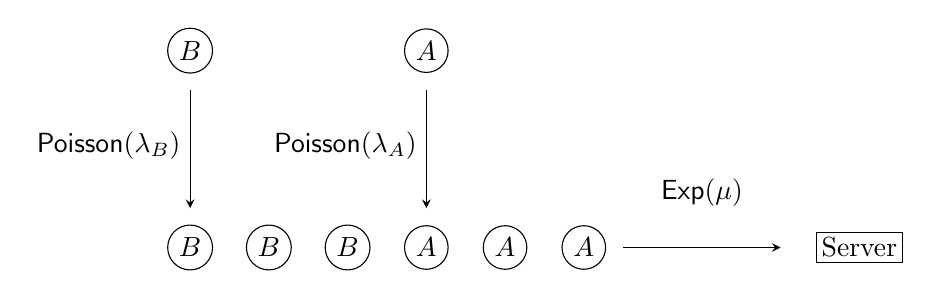
\begin{tikzpicture}[>=stealth]

% Draw the initial ball labeled B and arrow pointing down
\node[circle, draw, inner sep=2pt] (B0) at (0,0) {$\typeB$} ;
\draw[->] (0,-0.5) -- ++(0,-1.5);
\filldraw (0,-1.2) node[anchor=east] {$\Poisson(\rateB)$};

% Draw the initial ball labeled A and arrow pointing down
\node[circle, draw, inner sep=2pt] (A0) at (3,0) {$\typeA$};
\draw[->] (3,-0.5) -- ++(0,-1.5);
\filldraw (3,-1.2) node[anchor=east] {$\Poisson(\rateA)$};

% Draw the balls labeled B
\foreach \x in {0,...,2}
    \node[circle, draw, inner sep=2pt] (B\x) at (\x,-2.5) {$\typeB$};

% Draw the balls labeled A
\foreach \x/\label in {3/A, 4/A, 5/A}
    \node[circle, draw, inner sep=2pt] (A\x) at (\x,-2.5) {$\typeA$};

% Draw the arrow to the right
\draw[->] (5.5,-2.5) -- (7.5,-2.5);
\filldraw (6.5,-1.5) node[anchor=north] {$\Exp(\rateS)$};

\node[rectangle, draw, inner sep=2pt] (A0) at (8.5,-2.5) {Server};
\end{tikzpicture}
\end{center}

\noindent 
All parameters in the model are common knowledge and the queue is observable. 
When customers arrive, they decide whether to join the queue or balk. 
Moreover, when they are in the queue, they can  renege, before getting served.
However, only $\typeB$-customers renege because, unlike $\typeA$-customers, their position in the queue can get worse with the arrival of higher-priority customers. 

\subsection{Random Walks}
\label{suse:random-walk}

We now introduce some notation and some stochastic tools that will be used in the sequel to study the equilibrium and optimum of this model. 
\begin{definition} \label{de:P-and_E}
Consider a $\typeB$-customer (Bridget) who has $\nA$ $\typeA$-customers and $\nB$ $\typeB$-customers ahead of her.
We call $\Preward(\nA,\nB)$ the probability that Bridget is served, and   $\Etime(\nA,\nB)$ the expected total time that Bridget spends  in the system.
\end{definition}

Note that $\Preward(\nA,\nB)$ and $\Etime(\nA,\nB)$ depend on the the values $(\nA,\nB)$, the queueing system parameters, and the customers' strategies.

Given a $\typeB$-customer in the queue,  consider the birth-and-death process $\parens*{\ncustY_{\ttime}}_{\ttime\ge 0}$ that counts the number of people in the system who are ahead of this customer at any given time $\ttime \ge 0$.
This process increases by $1$ when an $\typeA$-customer joins the queue, and decreases by $1$ when a service gets completed. 

Let $\rtime_0=0$ and, for every $\round\geq 1$,  define
\begin{equation}
\label{eq:random-time}
\rtime_{\round}=\inf\braces*{\ttime>\rtime_{\round-1} \colon \text{ at time $\ttime$ either a $\typeA$-customer arrives or a service is completed}}.
\end{equation}
Then, for every $\round>0$, $\rtime_{\round}-\rtime_{\round-1}\sim \Exp(\rateA+\rateS)$, which implies 
\begin{equation}
\label{eq:expect-interarrival} 
\Expect(\rtime_{\round}-\rtime_{\round-1})=1/(\rateA+\rateS).
\end{equation}

We let $\ncust_{\round} \coloneqq \ncustY_{\rtime_{\round}}$ be the number of customers in the system at time $\rtime_{\round}$. 
The process $\parens*{\ncust_{\round}}_{\round\in\naturals}$ is a random walk with state space $\naturals$ such that $\ncust_{0} = \nAB$ and
\begin{equation}
\label{eq:random-walk} 
\ncust_{\round+1}
=
\begin{cases}
\ncust_{\round} + 1 & \text{with probability $\rateA/(\rateA+\rateS)$},\\
\ncust_{\round} - 1 & \text{with probability $\rateS/(\rateA+\rateS)$, if $\ncust_{\round}>0$},\\ 
\ncust_{\round} & \text{with probability $\rateS/(\rateA+\rateS)$,  if $\ncust_{\round} = 0$}.
\end{cases}
\end{equation} 
The following graph pictorially represents the above transition probabilities.

% \begin{center}
% \begin{tikzpicture}[->, >=stealth, auto, semithick, node distance=2cm]
% \tikzstyle{every state}=[fill=white,draw=black,text=black]

% \node[] (A) {0};
% \node[] (B) [right of=A] {1};
% \node[] (C) [right of=B] {2};
% \node[] (D) [right of=C] {};
% \node[] (E) [right of=D] {$\nAB$};
% \node[] (F) [right of=E] {$\nAB+1$};
% \node[] (G) [right of=F] {};

% \path (A) edge [loop below] node {$\frac{\rateS}{\rateA+\rateS}$} (A)
%       (A) edge [bend left, above] node {$\frac{\rateA}{\rateA+\rateS}$} (B)
%       (B) edge [bend left, below] node {$\frac{\rateS}{\rateA+\rateS}$} (A)
%       (B) edge [bend left, above] node {$\frac{\rateA}{\rateA+\rateS}$} (C)
%       (C) edge [bend left, below] node {$\frac{\rateS}{\rateA+\rateS}$} (B)
%       (C) edge [dashed, above] node {} (D)
%       (D) edge [dashed, above] node {} (E)
%       (D) edge [bend left, above] node {$\frac{\rateA}{\rateA+\rateS}$} (E)
%       (E) edge [bend left, below] node {$\frac{\rateS}{\rateA+\rateS}$} (D)
%       (E) edge [bend left, above] node {$\frac{\rateA}{\rateA+\rateS}$} (F)
%       (F) edge [bend left, below] node {$\frac{\rateS}{\rateA+\rateS}$} (E)
%       (F)  edge [dashed, above] node {} (G);

% \end{tikzpicture}
% \end{center}

\begin{center}
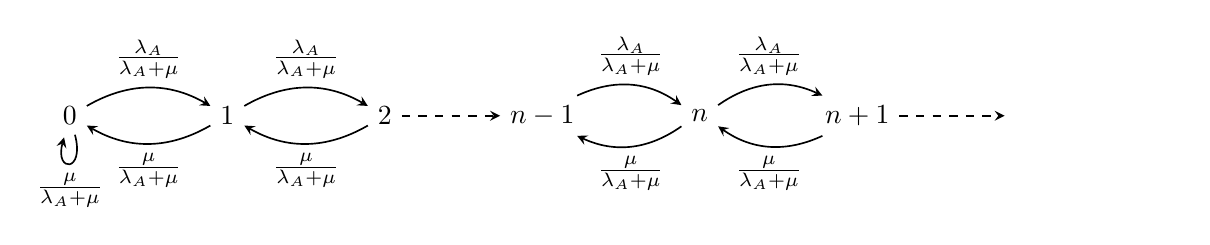
\begin{tikzpicture}[->, >=stealth, auto, semithick, node distance=2cm]
\tikzstyle{every state}=[fill=white,draw=black,text=black]

\node[] (A) {$0$};
\node[] (B) [right of=A] {$1$};
\node[] (C) [right of=B] {$2$};
\node[] (D) [right of=C] {$\nAB-1$};
\node[] (E) [right of=D] {$\nAB$};
\node[] (F) [right of=E] {$\nAB+1$};
\node[] (G) [right of=F] {};
\node[] (H) [right of=G] {};

\path (A) edge [loop below] node {$\frac{\rateS}{\rateA+\rateS}$} (A)
      (A) edge [bend left, above] node {$\frac{\rateA}{\rateA+\rateS}$} (B)
      (B) edge [bend left, below] node {$\frac{\rateS}{\rateA+\rateS}$} (A)
      (B) edge [bend left, above] node {$\frac{\rateA}{\rateA+\rateS}$} (C)
      (C) edge [bend left, below] node {$\frac{\rateS}{\rateA+\rateS}$} (B)
      (C) edge [dashed, above] node {} (D)
      (D) edge [bend left, above] node {$\frac{\rateA}{\rateA+\rateS}$} (E)
      (E) edge [bend left, below] node {$\frac{\rateS}{\rateA+\rateS}$} (D)
      (E) edge [bend left, above] node {$\frac{\rateA}{\rateA+\rateS}$} (F)
      (F) edge [bend left, below] node {$\frac{\rateS}{\rateA+\rateS}$} (E)
      (F)  edge [dashed, above] node {} (G);

\end{tikzpicture}
\end{center}



%
% Section ----------------------------------
%

\section{Semi-Strategic Model}
\label{se:semi-strategic}

To better understand the fully strategic model of the following sections, it is convenient to start our analysis with a ``semi-strategic'' regime where only $\typeB$-customers are strategic, whereas  $\typeA$-customers always join the queue and never renege. 
In this section, to guarantee stability of the system, we assume that $\rateS>\rateA$. 
At any given time, a $\typeB$-customer, knowing the state of the queue, decides to join the queue (or to remain in it), if and only if the expected future payoff of this customer is non-negative. 
The state of the queue is the pair $(\nA,\nB)$, representing the number of customers of type $\typeA$ and $\typeB$ who are already in the system, respectively. 
Let $(\nA,\nB)$ be the state of the system and let Bernard be the last $\typeB$-customer in the queue. 
Bernard can be served only when all the customers ahead of him have been served.
The number of these customers increases with each arrival of a new $\typeA$-customer.
Call $\benefitB(\nA,\nB)$ be the expected payoff for Bernard, when he is in position $\nAB=\nA+\nB$, and would renege when in position $\nAB+1$.  
Then $\benefitB(\nA,\nB)$ can be written as follows:
\begin{equation}
\label{eq:NetBenefit0}  \benefitB(\nA,\nB)=\rewardB \Preward(\nA,\nB-1)-\CostB \Etime(\nA,\nB-1).
\end{equation}
However, since $\typeA$-customers are not strategic and the service regime is \ac{FCFS}, the only relevant information for Bernard is the total number of customers $\nAB=\nA+\nB$ in the system. Hence $\benefitB(\nA,\nB)$ depends only on $\nAB$ and
\begin{equation}
\label{eq:NetBenefit}  \benefitB(\nA,\nB)\coloneqq\benefitnB(\nAB) = \rewardB \Preward_{\nAB}-\CostB \Etime_{\nAB},
\end{equation}
where $\Preward_{\nAB}$ and $\Etime_{\nAB}$ are  the probability of being served and the expected time spent in the system by Bernard when he is in position $\nAB$.

\begin{lemma}
\label{le:phi-n-B} 
For $\nAB\in\naturals$, 
\begin{equation}
\label{eq:Net-benefit}
\benefitnB(\nAB)=\rewardB\frac{1-\utilizationA}{1-\utilizationA^{\nAB+1}}-\frac{\CostB}{\rateS(1-\utilizationA)}\parens*{\frac{\nAB(1-\utilizationA)-\utilizationA(1-\utilizationA^{\nAB})}{1-\utilizationA^{\nAB+1}}}.
\end{equation}
\end{lemma}

\begin{proof}
Consider  \eqref{eq:NetBenefit}.
We now compute the probability $\Preward_{\nAB}$ that Bernard (in position $\nAB$) is served  before reneging (position $\nAB+1$). 
We can interpret $\Preward_{\nAB}$ as the ruin probability in the gambler ruin problem where the initial position is $\nAB$, the goal is $\nAB+1$ and the winning probability in each round equals $\rateA/(\rateS+\rateA)$. 
Then, by \cref{theo:GamblerRuin1},
\begin{equation}
\label{eq:P-n-1}
\Preward_{\nAB}=\frac{1-\utilizationA}{1-\utilizationA^{\nAB+1}}.  
\end{equation}

The total time $\Etime_{\nAB}$, spent in the system by Bernard when he is in position $\nAB$ corresponds to the expected number of rounds until the gambler is either ruined or reaches her goal. 
Then by  \cref{theo:GamblerRuin2}, 
\begin{align}
\Etime_{\nAB}&=\frac{1}{\rateS-\rateA}\parens*{\nAB-(\nAB+1)\utilizationA\frac{1-\utilizationA^{\nAB}}{1-\utilizationA^{\nAB+1}}}\nonumber\\
&=\frac{1}{\rateS-\rateA}\parens*{\frac{\nAB(1-\utilizationA^{\nAB+1})-(\nAB+1)\utilizationA(1-\utilizationA^{\nAB})}{1-\utilizationA^{\nAB+1}}}\nonumber\\
&=\frac{1}{\rateS(1-\utilizationA)}\parens*{\frac{\nAB(1-\utilizationA)-\utilizationA(1-\utilizationA^{\nAB})}{1-\utilizationA^{\nAB+1}}}. \nonumber
\end{align}
\end{proof}


%
% Subection ----------------------------------
%

\subsection{Equilibrium Strategy}\label{SubSec:SSEquilibrium}

In the following theorem, we characterize the equilibrium strategy for a $\typeB$-customer in the semi-strategic setup. 

\begin{theorem}
\label{theo:NetBenefitSemi-Strat}
Let $\nAB\in\naturals$ be the position in the queue of a $\typeB$-customer. 
The optimal strategy for this $\typeB$-customer 
% in a semi-strategic queueing regime with preemption 
is a threshold strategy, and the threshold $\Meq$ is the floor of the unique solution of the following equation:
\begin{equation}\label{eq:PriorityOptEquation}  \frac{\rewardB\rateS}{\CostB}=\frac{\nAB(1-\utilizationA)-\utilizationA(1-\utilizationA^{\nAB})}{(1-\utilizationA)^2}.
\end{equation}
\end{theorem}

\begin{proof}
The threshold is the largest  $\nAB$ for which $\benefitnB(\nAB)$ is nonnegative. 
By equation \eqref{eq:Net-benefit}, the threshold is the largest $\nAB$ such that
\begin{equation}
\label{eq:join-stay}  
\rewardB\frac{1-\utilizationA}{1-\utilizationA^{\nAB+1}}-\frac{\CostB}{\rateS(1-\utilizationA)}\parens*{\frac{\nAB(1-\utilizationA)-\utilizationA(1-\utilizationA^{\nAB})}{1-\utilizationA^{\nAB+1}}}\geq 0,
\end{equation}
which happens if and only if

\begin{equation}
\label{eq:B-joins}
\begin{split}    
\frac{\rewardB\rateS}{\CostB}
&\geq \frac{1-\utilizationA^{\nAB+1}}{(1-\utilizationA)^2}\cdot\frac{\nAB(1-\utilizationA)-\utilizationA(1-\utilizationA^{\nAB})}{1-\utilizationA^{\nAB+1}} \\
&=\frac{\nAB(1-\utilizationA)-\utilizationA(1-\utilizationA^{\nAB})}{(1-\utilizationA)^2}.
\end{split}
\end{equation}
If we let $\rhsBjoins(\nAB)$ denote the right hand side of \eqref{eq:B-joins}, then, the function $\rhsBjoins(\argdot)$ is unbounded and increasing, with $\rhsBjoins(0)=0$, so there exists a unique value $\Meq$ such that 
\begin{equation}
\label{eq:unique-value} \rhsBjoins(\Meq)\leq \frac{\rewardB\rateS}{\CostB}\leq \rhsBjoins(\Meq+1),   
\end{equation}
and $\Meq$ is the floor of the unique solution of $\rhsBjoins(\nAB)=\rewardB\rateS/\CostB$.
\end{proof}

The proofs of \cref{le:phi-n-B} and \cref{theo:NetBenefitSemi-Strat} resemble the proof of  \citet[lemma~2.4]{HasHav:Kluwer2003}, which deals with the social optimum threshold in  the Naor model. 
In fact, equations \eqref{eq:NaorOptEquation} and  \eqref{eq:PriorityOptEquation} differ only in the choice of rewards and costs. 
This is not surprising because, for a $\typeB$-customer, the semi-strategical priority regime is equivalent to a single-class \ac{LCFS} regime with arrival rate $\rateA$.



%
% Section ----------------------------------
%
\section{Fully-Strategic Model}
\label{se:fully-strategic}
We consider now a fully-strategic queueing regime  where all customers act strategically, independently of their type. 
Since $\typeA$-customers have priority over $\typeB$-customers, their behavior is not influenced by the arrival of $\typeB$-customers. Therefore, the equilibrium behavior of $\typeA$-customers is the same as in \citet{Nao:E1969}, \ie  they use a threshold strategy, where the threshold is given by
\begin{equation}
\label{eq:Naor}
\naor=\floor*{\frac{\rewardA\rateS}{\CostA}}.
\end{equation}
The threshold $\naor$ sets an upper bound on the number of $\typeA$-customers in the system. 
In the fully-strategic model the state is the pair  $(\nA,\nB)$, representing the number of customers of type $\typeA$ and $\typeB$ who are already in the system, respectively.
The behavior of $\typeB$-customers depends on the threshold strategy of $\typeA$-customers.
In the following sections we characterize the equilibrium strategy of a $\typeB$-customer.




%
% Subsection ----------------------------------
%

\subsection{Equilibrium}
\label{suse:equilibrium-preemption}
Consider  a fully-strategic priority queueing system where $(\nA, \nB)$ is the state of the system. 
We note that if the ratio $\rewardB/\CostB$ is not too large, then the $\typeB$-customers will leave the queue before the $\typeA$-customers reach their own equilibroium threshold.
To identify the value of $\rewardB/\CostB$ at which this occurs, we first analyze the situation in which a new $\typeB$-customer (Bernard) arrives and the state of the system is $(\naor,0)$, so there are no $\typeB$-customers in the queue, whereas the number of $\typeA$-customers is maximum. 
Given that the situation for Bernard can never become worse, if he decides to join the queue, he will remain in the system until his service is completed. 
Therefore, Bernard will join the queue if and only if 
\begin{equation}
\label{eq:FSNetBenefitIneq}
\rewardB-\CostB\Etime(\naor,0)\geq0,
\end{equation}
The inequality in \eqref{eq:FSNetBenefitIneq} implies that, if $\rewardB/\CostB<\Etime(\naor,0)$, then a $\typeB$-customer in the queue will abandon the system before it reaches the state $\nA=\naor$. 

\begin{theorem}
\label{theo:ThresholdFS1}    
Consider a fully-strategic priority queueing regime. 
Let $(\nA,\nB)$ be the state of the system. 
If $\rewardB/\CostB<\Etime(\naor,0)$, then the optimal strategy for a $\typeB$-customer is a threshold strategy on the total number of customers $\nAB=\nA+\nB$. 
Moreover, the threshold is $\floor{\nunsol}$ where $\nunsol$ is the unique solution of the following equation
\begin{equation} \label{eq:thresholdeqFS1}
\frac{\rewardB\rateS}{\CostB}=
\begin{cases} \displaystyle{\frac{(\nAB+1)(1-\utilizationA)-\utilizationA(1-\utilizationA^{\nAB+1})}{(1-\utilizationA)^2}} & \text{ if } \utilizationA\neq 1 \\ 
\\
\displaystyle{\frac{(\nAB+1)(\nAB+2)}{2}}& \text{ if } \utilizationA=1.
\end{cases}
\end{equation}    
\end{theorem}

The proof of \cref{theo:ThresholdFS1} is similar to that of \cref{theo:NetBenefitSemi-Strat}. 
In fact,  \cref{eq:thresholdeqFS1} coincides with  \cref{eq:PriorityOptEquation}, except that $\nAB$ is replaced by $\nAB+1$. 
This is due to the fact that, in \cref{theo:ThresholdFS1}, the new $\typeB$-customer would enter position $\nAB+1$, whereas in \cref{theo:NetBenefitSemi-Strat}, Bernard was already in the queue at position $\nAB$.

Moreover, the threshold given by \eqref{eq:thresholdeqFS1} is smaller than $\naor$.
This can be proved with the aid of \cref{le:E-time}, which shows that  the condition $\rewardB/\CostB<\Etime(\naor,0)$ can be written as follows:
\begin{equation}    \frac{\rewardB\rateS}{\CostB}<
\begin{cases}
\displaystyle{       \frac{(\naor+1)(1-\utilizationA)-\utilizationA\parens*{1-\utilizationA^{\naor+1}}}{(1-\utilizationA)^2}} & \text{ if } \utilizationA\neq 1\\ \\ 
\displaystyle{\frac{(\naor+1)(\naor+2)}{2}} & \text{ if } \utilizationA=1.
    \end{cases}
\end{equation}

Now we focus on the case  $\rewardB/\CostB\geq\Etime(\naor,0)$. 

\begin{theorem}
\label{theo:OptThresholdB-customers}
Consider a fully-strategic queueing system. 
Assume that   $(\nA,\nB)$ is the state of the system, and  $\rewardB/\CostB\geq \Etime(\naor,0)$. 
A $\typeB$-customer joins the queue if $\nAB=\nA+\nB<\Teq$, where
\begin{equation}
\label{eq:BThresholdStrat}
\Teq\coloneqq\naor+\Veq,
\end{equation}
and
\begin{equation}
\label{eq:Threshold-FS-Bcustomer}
\Veq=
\begin{cases}
\displaystyle{\floor*{\frac{1-\utilizationA}{1-\utilizationA^{\naor+1}}\bracks*{\frac{\rewardB\rateS}{\CostB}-\frac{1}{1-\utilizationA}\parens*{\naor-\frac{\utilizationA}{1-\utilizationA}\parens*{1-\utilizationA^{\naor}}}}}} & \text{ if } \utilizationA\neq 1, \\ \\ 
\displaystyle{\floor*{\frac{\rewardB\rateS}{\CostB(\naor+1)}-\frac{\naor}{2}}} 
& \text{ if } \utilizationA=1. \end{cases}
\end{equation}
\end{theorem}

\begin{proof}
If $\rewardB/\CostB\geq \Etime(\naor,0)$, the first $\typeB$-customer always joins the queue. 
We now determine the  maximum number of $\typeB$-customers that will always join the queue. 
To answer this question we consider the worst-case scenario, \ie we assume that the state of the system is $(\naor,\nB)$, and prove that, if $\rewardB/\CostB\geq \Etime(\naor,0)$, then a new $\typeB$-customer joins the queue whenever $\nB<\Veq$.
 
If the state is $(\naor,\nB)$, as time goes by, the situation for a new $\typeB$-customer who joins the queue can only improve; therefore this customer will join if
\begin{equation}
\label{eq:Bjoinqueue}
    \rewardB-\CostB\Etime(\naor,\nB)\geq 0.
\end{equation}
By  \cref{le:E-time}, if $\utilizationA\neq 1$,  then \eqref{eq:Bjoinqueue} is equivalent to

\begin{align}
&\rewardB\geq\CostB\frac{1}{\rateS(1-\utilizationA)} \bracks*{(\nB+1)\parens*{1 - \utilizationA^{\naor+1}}+  \naor-\frac{\utilizationA^{\naor+1}}{1-\utilizationA} \parens*{\utilizationA^{-\naor}-1}},
\intertext{that is,}
&\frac{\rewardB\rateS}{\CostB}\geq (\nB+1)\frac{1-\utilizationA^{\naor+1}}{1-\utilizationA}+\frac{1}{1-\utilizationA}\parens*{\naor-\frac{\utilizationA}{1-\utilizationA}\parens*{1-\utilizationA^{\naor}}},
\intertext{which becomes}
&\frac{1-\utilizationA}{1-\utilizationA^{\naor+1}}\bracks*{\frac{\rewardB\rateS}{\CostB}-\frac{1}{1-\utilizationA}\parens*{\naor-\frac{\utilizationA}{1-\utilizationA}\parens*{1-\utilizationA^{\naor}}}}\geq\nB+1, 
\intertext{and, finally}
&\frac{1-\utilizationA}{1-\utilizationA^{\naor+1}}\bracks*{\frac{\rewardB\rateS}{\CostB}-\frac{\naor(1-\utilizationA)-\utilizationA\parens*{1-\utilizationA^{\naor}}}{(1-\utilizationA)^2}}\geq \nB +1.
\end{align}

If $\utilizationA=1$, again, by  \cref{le:E-time},    \cref{eq:Bjoinqueue} is equivalent to
\begin{align}
&\rewardB\geq\CostB\frac{1}{2\rateS}\bracks*{\naor(\naor+1)+2(\nB+1)(\naor+1)},
\intertext{that is,}
&\frac{2\rewardB\rateS}{\CostB(\naor+1)}\geq2(\nB+1)+\naor,
\intertext{which is the same as}
&\frac{\rewardB\rateS}{\CostB(\naor+1)}-\frac{\naor}{2}\geq\nB+1.
\end{align}

Hence, if the state of the system is $(\naor,\nB)$, then a $\typeB$-customer joins the queue if $\nB<\Veq$, where $\Veq$ is given by \eqref{eq:Threshold-FS-Bcustomer}.

Combining the thresholds in \cref{eq:Threshold-FS-Bcustomer,eq:Naor}, we see that the number of customers in the system cannot exceed $ \naor+\Veq$. 
We now show that this value represents the optimal threshold strategy for a $\typeB$-customer in a fully-strategic queueing model when $\rewardB/\CostB\geq \Etime(\naor,0)$.

Let now $(\nA,\nB)$ be the state of the system. 
By \eqref{eq:Naor} and \eqref{eq:Threshold-FS-Bcustomer}, $\nAB=\nA+\nB$ cannot be larger than $\Teq$. 
Moreover, if $\nA\leq\naor$, we proved  that a $\typeB$-customer joins the queue whenever $\nB<\Veq$, and in this case, $\nAB$ is smaller than $\Teq$. 
We now consider the case $ \nB \geq \Veq $.
Since $ \nAB < \Teq $, the value $\nA$ must be smaller than $\naor$; therefore a new $\typeB$-customer (Brianna) joins the queue if 
\begin{equation}
\rewardB\Preward(\nA,\nB)-\CostB\Etime(\nA,\nB)\geq0,
\end{equation}
where $\Preward(\nA,\nB)$ is the probability that Brianna completes the service before reneging (position $ \Teq + 1 $), and $\Etime(\nA,\nB)$ is the expected total time spent in the system by Brianna, when the state of the system is $(\nA,\nB)$.

We can interpret $\Preward(\nA,\nB)$ as the ruin probability in the gambler ruin problem that we now describe.
We consider a random walk on $\naturals^{2}$ with the following transition probabilities:
\begin{equation}
\label{eq:random-walk-1} 
\begin{split}
&\text{for }\nA=0,\\
&(\nA,\nB) \to  (\nA+1,\nB)  \quad\text{w.p.\ } \frac{\rateA}{\rateA+\rateS},\quad
(\nA,\nB) \to  (\nA,\nB-1)  \quad\text{w.p.\ } \frac{\rateS}{\rateA+\rateS},\\ 
&\text{for }0< \nA<\naor,\\
&(\nA,\nB) \to  (\nA+1,\nB)  \quad\text{w.p.\ } \frac{\rateA}{\rateA+\rateS},\quad
(\nA,\nB) \to  (\nA-1,\nB)  \quad\text{w.p.\ } \frac{\rateS}{\rateA+\rateS},\\
&\text{for }\nA=\naor,\\
&(\nA,\nB) \to  (\nA,\nB)  \quad\text{w.p.\ } \frac{\rateA}{\rateA+\rateS},\quad
(\nA,\nB) \to  (\nA-1,\nB)  \quad\text{w.p.\ } \frac{\rateS}{\rateA+\rateS}.
\end{split}
\end{equation}
The transitions are represented in \cref{fig:ruin-1}.
Notice that, even if the random walk is on $\naturals^{2}$, in every state, a transition occurs with positive probability only to two adjacent states.
So this random walk is equivalent to a single dimensional random walk.

\bigskip
\begin{figure}[h!]

\begin{tikzpicture}[scale=1.2]

% Disegno del sistema cartesiano (solo la parte positiva)
\draw[->] (0,0) -- (8,0) node[anchor=north] {$\nA$}; % Asse x
\draw[->] (0,0) -- (0,8) node[anchor=east] {$\nB$};  % Asse y

% Retta verticale spostata a x=4
\draw[red,thick] (4,0) -- (4,2); % Parte piena fino all'intersezione
\draw[red, dashed] (4,2) -- (4,8); % Parte tratteggiata sopra l'intersezione
\node[below] at (4,0) {$\naor$}; % Etichetta del punto $\optA$

% Segmento obliquo partente da (0,6) a (6,0)
\draw[blue,thick] (0,6) -- (4,2); % Parte rossa fino all'intersezione
\draw[blue,dashed] (4,2) -- (6,0); % Parte tratteggiata dopo l'intersezione

% Retta orizzontale che va dall'asse y fino al punto di intersezione
\draw[thick] (0,2) -- (4,2); % Segmento orizzontale non tratteggiato

% Aggiungo il reticolo tratteggiato nel trapezio
\foreach \y in {0, 1, 2} { % Linee orizzontali
    \draw[dashed] (0,\y) -- (4,\y);
}
\foreach \y in {3, 4, 5, 6} { % Linee orizzontali
    \draw[dashed] (0,\y) -- (6-\y,\y);
}
\foreach \x in {0, 1, 2, 3, 4} { % Linee verticali
    \draw[dashed] (\x,0) -- (\x,6-\x);
}

% Punto e etichetta per $\nAB$
\node[left] at (0,6) {$\Teq$};
\node[left] at (0,2) {$\Veq$};
\node[left] at (0,0) {$(0,0)$};

% Aggiungo punti marcati per chiarezza
\fill (0,6) circle (2pt); % Punto (0,6)
\fill (4,2) circle (2pt); % Punto d'intersezione
\fill (4,0) circle (2pt); 
\fill (0,2) circle (2pt); 
\fill (0,0) circle (2pt); 

% Aggiungi le frecce a partire dal punto (4,1)
\draw[->] (4,1) -- (3.1,1); % Freccia verso sinistra
\node[below] at (3.5,1) {$\rateS$};
\path (4,1) edge [loop right] node {$\rateA$} (4,1);

% Aggiungi le frecce a partire dal punto (2,1)
\draw[->] (2,1) -- (2.9,1); % Freccia verso destra
\node[below] at (2.5,1) {$\rateA$};
\draw[->] (2,1) -- (1.1,1); % Freccia verso sinistra
\node[below] at (1.5,1) {$\rateS$};


% Aggiungi le frecce a partire dal punto (0,1)
\draw[->] (0,1) -- (0.9,1); 
\node[below] at (0.5,1) {$\rateA$};
\draw[->] (0,1) -- (0,0.1); 
\node[left] at (0,0.5) {$\rateS$};


% Aggiungi le frecce a partire dal punto (0,4)
\draw[->] (0,4) -- (0.9,4); 
\node[below] at (0.5,4) {$\rateA$};
\draw[->] (0,4) -- (0,3.1); 
\node[left] at (0,3.5) {$\rateS$};


% Aggiungi le frecce a partire dal punto (2,3)
\draw[->] (2,3) -- (2.9,3); % Freccia verso destra
\node[below] at (2.5,3) {$\rateA$};
\draw[->] (2,3) -- (1.1,3); % Freccia verso sinistra
\node[below] at (1.5,3) {$\rateS$};

\end{tikzpicture}

\caption{Random-walk representation of a $\typeB$-customer strategy}
  \label{fig:ruin-1}
\end{figure}

Once Brianna reaches the position $(0,\Veq)$, she gets served with probability $1$.
Hence, by \cref{theo:GamblerRuin1},
\begin{equation}
\label{eq:P-n-2}
\Preward(\nA,\nB)=
\begin{cases}
\displaystyle{\frac{1-\utilizationA^{\Teq-\nAB}}{1-\utilizationA^{\naor+1}}} & \text{ if } \utilizationA\neq 1 \\ \\ 
\displaystyle{\frac{\Teq-\nAB}{\naor+ 1}} &\text{ if } \utilizationA= 1.\end{cases}
\end{equation}
The expected total time $\Etime(\nA,\nB)$ spent in the system by Brianna can be interpreted as the expected time before  the first arrival either at $(0,0)$ or at $(\nA,\Teq-\nA+1)$. 
Then, it is possible to decompose $\Etime(\nA,\nB)$ in the following way

    \begin{equation}
        \Etime(\nA,\nB)=\Exittime(\nA,\nB)+ \Preward(\nA,\nB)\Etime(0,\Veq-1),
    \end{equation}
where $\Exittime(\nA,\nB)$ is the expected time of first arrival in either $(0,\Veq)$ or $(\nA,\Teq-\nA+1)$  starting from position $\nAB+1$; whereas $\Etime(0,\Veq-1)$,  is the expected waiting time spent by Brianna's in the system  when there are $(0,\Veq-1)$ customers ahead of her.


Then, by \cref{theo:GamblerRuin2},
\begin{equation}
\Exittime(\nA,\nB)=
\begin{cases}
\displaystyle{\frac{(\nAB+1-\Veq)\parens*{1-\utilizationA^{\naor+1}}-(\naor+1)\parens*{\utilizationA^{\Teq-\nAB}-\utilizationA^{\naor+1}}}{\rateS(1-\utilizationA)\parens*{1-\utilizationA^{\naor+1}}}} & \text{ if } \utilizationA\neq 1 \\ \\ \displaystyle{\frac{(\nAB+1-\Veq)(\Teq-\nAB)}{2\rateS}}
&\text{ if } \utilizationA= 1.
\end{cases}
\end{equation}
Moreover, by \cref{le:E-time},
    \begin{equation}
        \Etime(0,\Veq-1)=\begin{cases}\frac{\Veq(1-\utilizationA^{\naor+1})}{\rateS(1-\utilizationA)} & \text{ if } \utilizationA\neq 1 \\ \\
        \frac{\Veq}{\rateS}(\naor+1) &\text{ if } \utilizationA= 1.         
        \end{cases}
    \end{equation}
Hence, if $\utilizationA=1$, Brianna joins the queue if
\begin{equation}
\label{eq:Brianna-joins}   
\begin{split}
\frac{\rewardB}{\CostB}
&\geq  
\frac{(\nAB+1-\Veq)(\naor+1)}{2\rateS}+ \frac{\Veq}{\rateS}(\naor+1) \\
&= 
\frac{\naor+1}{2\rateS}\parens*{ \nAB+1 +\Veq},
\end{split}
\end{equation}
that is,
\begin{equation}
\label{eq:Brianna-joins-2} 
\frac{\rewardB}{\CostB}\cdot\frac{2\rateS}{\naor+1}-\Veq\geq \nAB+1.
\end{equation}
So, by \eqref{eq:Threshold-FS-Bcustomer}, Brianna joins the queue if $\nAB+1\leq \Teq$.
  
If $\utilizationA\neq 1$, Brianna joins the queue if
\begin{equation}
\label{eq:Brianna-joins-rho-not-1}  
\frac{\rewardB}{\CostB}\geq \frac{(\nAB+1-\Veq)\parens*{1-\utilizationA^{\naor+1}}-(\naor+1)\parens*{\utilizationA^{\Teq-\nAB}-\utilizationA^{\naor+1}}}{\rateS(1-\utilizationA)\parens*{1-\utilizationA^{\Teq-\nAB}}} +\frac{\Veq\parens*{1-\utilizationA^{\naor+1}}}{\rateS(1-\utilizationA)}.
\end{equation}
By equation \eqref{eq:Threshold-FS-Bcustomer} this is equivalent to
\begin{equation}
\label{eq:Brianna-joins-rho-not-1-a} 
\begin{split}
\frac{\rewardB}{\CostB}
&\geq \frac{(\nAB+1-\Veq)\parens*{1-\utilizationA^{\naor+1}}-(\naor+1)\parens*{\utilizationA^{\Teq-\nAB}-\utilizationA^{\naor+1}}}{\rateS(1-\utilizationA)\parens*{1-\utilizationA^{\Teq-\nAB}}} \\
&\quad+\frac{\rewardB}{\CostB}-\frac{\naor}{\rateS(1-\utilizationA)}+ \frac{\utilizationA(1-\utilizationA^{\naor})}{\rateS(1-\utilizationA)^2},
\end{split}
\end{equation}
That is
\begin{equation}
\label{eq:Brianna-joins-rho-not-1-b} 
\begin{split}
0
&\geq \frac{(\nAB+1-\Veq)\parens*{1-\utilizationA^{\naor+1}}-(\naor+1)\parens*{\utilizationA^{\Teq-\nAB}-\utilizationA^{\naor+1}}}{\rateS(1-\utilizationA)\parens*{1-\utilizationA^{\Teq-\nAB}}} \\
&\quad+ \frac{\utilizationA(1-\utilizationA^{\naor})-\naor(1-\utilizationA)}{\rateS(1-\utilizationA)^2}.
\end{split}
\end{equation}

Define 
\begin{equation}
\label{eq:G(n)}    G(\nAB)=\frac{(\nAB+1-\Veq)\parens*{1-\utilizationA^{\naor+1}}-(\naor+1)\parens*{\utilizationA^{\Teq-\nAB}-\utilizationA^{\naor+1}}}{\rateS(1-\utilizationA)\parens*{1-\utilizationA^{\Teq-\nAB}}}.
\end{equation}

\begin{claim}
\label{cl:G-increasing} 
The function $\nAB\mapsto G(\nAB)$ is increasing for $\Veq\leq \nAB \leq \Teq-1$.
\end{claim}
\begin{proof}
See \cref{se:appendix-proofs}.    
\end{proof}
Hence, if we take $\nAB=\Teq-1$ we have
\begin{equation}
\label{eq:0=0}   \begin{split}
0
&\geq \frac{\naor\parens*{1-\utilizationA^{\naor+1}}-(\naor+1)\utilizationA\parens*{1-\utilizationA^{\naor}}+\utilizationA(1-\utilizationA^{\naor})-\naor(1-\utilizationA)}{\rateS(1-\utilizationA)^2}\\
&= \frac{\naor\parens*{1-\utilizationA}-\utilizationA\parens*{1-\utilizationA^{\naor}}+\utilizationA(1-\utilizationA^{\naor})-\naor(1-\utilizationA)}{\rateS(1-\utilizationA)^2}\\
&=0.     
\end{split} 
\end{equation}
Then, the Brianna joins whenever $\nAB<\Teq$.
\end{proof}

\begin{remark}
\label{re:observanle-n}
In the whole paper, queues are assumed to be observable. 
It is important to clarify that if Abigail is an $\typeA$-customer and Bernard is a $\typeB$-customer, they can make their equilibrium decision by observing just the other customers that are (potentially) ahead of them, in the queue. 
That is, when Abigail arrives at the queue, all she needs to know is how many $\typeA$-customers are already in the queue. 
She does not case about $\typeB$-customers, because they will never be ahead of her. 
When Bernard arrives at the queue or, if he already is in the queue, he can make his balking or reneging equilibrium decisions based on the total number of customers ahead of him in the queue.
He does not need to know their types.

\end{remark}





%
% Section ----------------------------------
%
    

\section{Global Optimization}
\label{se:global-optimization}
In the previous section we analyzed the  equilibrium behavior of selfish  customers both in semi-strategic and fully strategic frameworks. 
We now focus on socially optimum behavior. 
We assume the existence of a social planner who obtains a reward $\rewardA$ for any completed service of an $\typeA$-customer,  a reward $\rewardB$ for any completed service of a $\typeB$-customer, and incurs a cost $\CostA$ for any unit of time spent in the system by an $\typeA$-customer and a  cost $\CostB$ for any unit of time spent in the system by a $\typeB$-customer.
The social planner has full discretion and can decide whom to accept in the queue and whom to kick out, without any priority constraints. 
It is clear that the social planner has an incentive to favor customers whose reward-to-cost ratio $\rewardtype/\Costtype$ is higher. 
For instance, if $\rewardA/\CostA>\rewardB/\CostB$, then the social planner will admit at most 
$\optA=\floor{\nA^*}$ customers in the system, where $\nA^*$ is the unique solution of the equation 
\begin{equation}
\label{eq:opt-Naor-A}  
\frac{\rewardA\rateS}{\CostA}=
\begin{cases} 
\displaystyle{\frac{\nA^*(1-\utilizationA)-\utilizationA(1-\utilizationA^{\nA^*})}{(1-\utilizationA)^2}} 
& \text{ if } \utilizationA \neq 1,\\ 
\\
\displaystyle{\frac{\nA(\nA+1)}{2}} 
&\text{ if } \utilizationA = 1.
\end{cases}
\end{equation}
If $\nA<\optA$, the planner can accept a number of $\typeB$-customers.
Given $\nA$, the optimum total number of customers that can be admitted can be found by imposing a \ac{LCFS} regime  the customers'  equilibrium behavior. 
This is the technique used by \citet{Has:E1985} to determine the social optimum in the model with a single class.
The idea is that in a \ac{LCFS} regime the decision made by the last customer in the queue does not generate any externality on the other customers. 
Therefore what is optimal for this customer is also socially optimal.

If we define $\utilization \coloneqq (\rateA+\rateB)/\rateS$, then the optimum threshold on $\nA+\nB$ for the admission of a $\typeB$-customer is $\floor*{\nAB^{*}}$, where $\nAB^{*}$ is the unique solution of the equation
\begin{equation}
\label{eq:opt-threshold-B-tot}    
\frac{\rewardB\rateS}{\CostB}=
\begin{cases}
\displaystyle{\frac{\nAB^*(1-\utilization)-\utilization(1-\utilization^{\nAB^*})}{(1-\utilization)^2}} 
&\text{ if } \utilization\neq 1 \\
\\
\displaystyle{\frac{\nAB^*(\nAB^*+1)}{2}}
&\text{ if } \utilization=1. 
\end{cases}
\end{equation}
The above result implies that, if $\nA<\optA$, and a new $\typeA$-customer arrives, whenever the total number of customers (including the newcomer) exceeds $\floor*{\nAB^{*}}$, a $\typeB$-customer will be forced to renege.



%
% Section ----------------------------------
%

\section{Class Optimization}
\label{se:class-optimization}
We consider now the case where priorities are binding even for social planners.
We represent this situation by assuming that there exist two social planners, one for each type. 
As in the previous section, for $\type$ in $\braces*{\typeA,\typeB}$, the $\type$-planner receives a reward $\rewardtype$ for each completed service of a $\type$-customer and incurs a cost $\Costtype$ for each unit of time a $\type$-customer spends in the system. 

First we analyze the optimal strategy for the $\typeA$-planner (Anastasia-Paris). 
Since $\typeA$-customers are not influenced by $\typeB$-customers, this is the classical optimal control problem of the Naor model. 
Thus, as seen in the previous section, Anastasia-Paris's threshold is the following: 

\begin{theorem}
\label{theo:AClassOpt}
The optimal strategy for an $\typeA$-planner is a threshold strategy and the threshold is 
\begin{equation}
\label{eq:AClassOpt}
\optA=\floor*{\nA^*},    \end{equation}
where $\nA^*$ is the unique solution of     \begin{equation} \frac{\rewardA\rateS}{\CostA}=
\begin{cases} 
\displaystyle{\frac{\nA^*(1-\utilizationA)-\utilizationA(1-\utilizationA^{\nA^*})}{(1-\utilizationA)^2}} 
& \text{ if } \utilizationA \neq 1,\\ 
\\
\displaystyle{\frac{\nA(\nA+1)}{2}} 
&\text{ if } \utilizationA = 1.
\end{cases}
\end{equation}
\end{theorem}

We now consider the optimal strategy for the $\typeB$-planner (Belinda-Paris), who knows the optimal strategy of Anastasia-Paris. 
Along the lines of  \citet{Has:E1985}, it can be shown that Belinda-Paris's optimal strategy coincides with the  equilibrium strategy in a \ac{LCFS} regime. 
However, in our case, the $\typeB$-customers' equilibrium strategy depends on $\optA$.
If $\rewardB/\CostB < \rewardA/\CostA$, then Belinda-Paris's optimal strategy  coincides with the strategy used by the unique social planner. 
Hence,  we focus on Belinda-Paris's  optimal strategy when $\rewardB/\CostB \ge  \rewardA/\CostA$. 
In this situation,  Belinda-Paris may accept $\typeB$-customers even if there are $\optA$ $\typeA$-customers in the queue. 
Thus, as already done for the equilibrium strategy, we assume that the state is $(\nA,\nB)$, that the last $\typeB$-customer (Benjamin) is in position $\nAB = \nA + \nB > \optA$, and that he will renege when in position $\nAB + 1$.
Unlike the equilibrium case, however, now Benjamin's position can become worse even after the arrival of another $\typeB$-customer. 
Hence, to find the optimal strategy we have to compute the largest values $\nAB$ such that
\begin{equation}
\label{eq:Benjamin}  
\rewardB\Preward(\nA,\nB-1)-\CostB\Etime(\nA,\nB-1)\geq0,
\end{equation}

It is possible to compute $\Preward(\nA,\nB-1)$ and $\Etime(\nA,\nB-1)$ by describing the problem as a random walk.

\bigskip
\begin{figure}[h!]

\begin{tikzpicture}[scale=1.2]

% Disegno del sistema cartesiano (solo la parte positiva)
\draw[->] (0,0) -- (8,0) node[anchor=north] {$\nA$}; % Asse x
\draw[->] (0,0) -- (0,8) node[anchor=east] {$\nB$};  % Asse y

% Retta verticale spostata a x=4
\draw[red,thick] (4,0) -- (4,2); % Parte piena fino all'intersezione
\draw[red, dashed] (4,2) -- (4,8); % Parte tratteggiata sopra l'intersezione
\node[below] at (4,0) {$\optA$}; % Etichetta del punto $\optA$

% Segmento obliquo partente da (0,6) a (6,0)
\draw[blue,thick] (0,6) -- (4,2); % Parte rossa fino all'intersezione
\draw[blue,dashed] (4,2) -- (6,0); % Parte tratteggiata dopo l'intersezione

% Retta orizzontale che va dall'asse y fino al punto di intersezione
\draw[thick] (0,2) -- (4,2); % Segmento orizzontale non tratteggiato

% Aggiungo il reticolo tratteggiato nel trapezio
\foreach \y in {0, 1, 2} { % Linee orizzontali
    \draw[dashed] (0,\y) -- (4,\y);
}
\foreach \y in {3, 4, 5, 6} { % Linee orizzontali
    \draw[dashed] (0,\y) -- (6-\y,\y);
}
\foreach \x in {0, 1, 2, 3, 4} { % Linee verticali
    \draw[dashed] (\x,0) -- (\x,6-\x);
}

% Punto e etichetta per $\nAB$
\node[left] at (0,6) {$\nAB$};
\node[left] at (0,2) {$\nAB-\optA$};
\node[left] at (0,0) {$(0,0)$};

% Aggiungo punti marcati per chiarezza
\fill (0,6) circle (2pt); % Punto (0,6)
\fill (4,2) circle (2pt); % Punto d'intersezione
\fill (4,0) circle (2pt); 
\fill (0,2) circle (2pt); 
\fill (0,0) circle (2pt); 

% Aggiungi le frecce a partire dal punto (4,1)
\draw[->,red] (4,1) -- (4,1.9); % Freccia verso l'alto
\node[right] at (4,1.5) {$\rateB$};
\draw[->] (4,1) -- (3.1,1); % Freccia verso sinistra
\node[below] at (3.5,1) {$\rateS$};
\path (4,1) edge [loop right] node {$\rateA$} (4,1);

% Aggiungi le frecce a partire dal punto (2,1)
\draw[->] (2,1) -- (2.9,1); % Freccia verso destra
\node[below] at (2.5,1) {$\rateA$};
\draw[->] (2,1) -- (1.1,1); % Freccia verso sinistra
\node[below] at (1.5,1) {$\rateS$};
\draw[->] (2,1) -- (2,1.9); % Freccia verso alto
\node[right] at (2,1.5) {$\rateB$};

% Aggiungi le frecce a partire dal punto (0,1)
\draw[->] (0,1) -- (0.9,1); 
\node[below] at (0.5,1) {$\rateA$};
\draw[->] (0,1) -- (0,0.1); 
\node[left] at (0,0.5) {$\rateS$};
\draw[->] (0,1) -- (0,1.9); 
\node[left] at (0,1.5) {$\rateB$};

% Aggiungi le frecce a partire dal punto (0,4)
\draw[->] (0,4) -- (0.9,4); 
\node[below] at (0.5,4) {$\rateA$};
\draw[->] (0,4) -- (0,3.1); 
\node[left] at (0,3.5) {$\rateS$};
\draw[->] (0,4) -- (0,4.9); 
\node[left] at (0,4.5) {$\rateB$};

% Aggiungi le frecce a partire dal punto (2,3)
\draw[->] (2,3) -- (2.9,3); % Freccia verso destra
\node[below] at (2.5,3) {$\rateA$};
\draw[->] (2,3) -- (1.1,3); % Freccia verso sinistra
\node[below] at (1.5,3) {$\rateS$};
\draw[->] (2,3) -- (2,3.9); % Freccia verso alto
\node[right] at (2,3.5) {$\rateB$};
\end{tikzpicture}
  \caption{Random-walk representation of a $\typeB$-planner strategy}
  \label{fig:ruin-2}
\end{figure}

As shown in \cref{fig:ruin-2},   $\Preward(\nA,\nB-1)$ represents the probability of reaching the vertex $(0,0)$ before exiting the trapezoid, starting from a point on the blue segment $(\nA,\nAB-\nA)$.
Analogously to the equilibrium case, to reach the point $(0,0)$ the random walk must pass through the point $(0,\nAB-\optA)$.
However, reaching this point does not guarantee service because the regime  is \ac{LCFS}. Similarly, $\Etime(\nA,\nB-1)$ represents the expected time before the random walk reaches $(0,0)$ or exits the trapezoid, starting from a point on the blue segment. 
Again, calculating the expected time is more complicated than in the previous sections, because, even after reaching the rectangle in the figure, the random walk may return to the triangle before reaching the point $(0,0)$. 
Just as we observed  in the equilibrium case, it is possible to obtain $\Preward(\nA,\nB-1)$ and $\Etime(\nA,\nB-1)$ as the solution of a system of equations, but in this case finding the solution in closed form is quite complicated.

For every $(\statei,\statej)$ in the trapezoid in \cref{fig:ruin-2}, we call  $\hitzero(\statei,\statej)$ the probability of reaching $(0,0)$ before leaving the trapezoid. Then, we can write $\Preward(\nA,\nB-1)$ as follows:


\begin{equation}
\Preward(\nA,\nB-1)=
\begin{cases} \displaystyle{\frac{1-\utilization}{1-\utilization^{\optA+1}}\hitzero(0,\nAB-\optA)} &\text{ if } \utilization\neq 1 \\ 
\\
\displaystyle{\frac{1}{\optA+1}\hitzero(0,\nAB-\optA)} & \text{ if } \utilization=1,\end{cases} \end{equation}
where $(1-\utilization)/(1-\utilization^{\optA+1})$ and $1/(\optA+1)$ are the probabilities of reaching $(0,\nAB-\optA)$ before leaving the triangle, starting from the blue segment $(\nA,\nAB-\nA)$. 
Moreover, by \cref{Theo:hittingTime} $\hitzero(0,\nAB-\optA)$ is obtained by the following system of equations:
\begin{align*}
\label{eq:etan-MA}
\begin{alignedat}{2}
\hitzero(0,0)
&=1,\\
\hitzero(0,\nAB-\optA)
&=\frac{\rateS}{\rate+\rateS}\hitzero(0,\nAB-\optA-1)+\frac{\rateA}{\rate+\rateS}\hitzero(1,\nAB-\optA)\\
&\quad+\frac{\rateB}{\rate+\rateS}\hitzero(0,\nAB-\optA+1),\\
\hitzero(0,\statej)
&=\frac{\rateS}{\rate+\rateS}\hitzero(0,\statej-1) +\frac{\rateA}{\rate+\rateS}\hitzero(1,\statej)+\frac{\rateB}{\rate+\rateS}\hitzero(0,\statej+1), \\
&\quad \text{ if } \statej<\nAB-\optA,\\
\hitzero(\optA,\nAB-\optA)
&= \frac{\rateS}{\rate+\rateS}\hitzero(\optA-1,\nAB-\optA)+\frac{\rateA}{\rate+\rateS}\hitzero(\optA,\nAB-\optA),\\
\hitzero(i,\nAB-\optA)
&=\frac{\rateS}{\rate+\rateS}\hitzero(\statei-1,\nAB-\optA)+\frac{\rateA}{\rate+\rateS}\hitzero(\statei+1,\nAB-\optA)\\
&\quad +\frac{\rateB}{\rate+\rateS}\hitzero(\statei,\nAB-\optA+1),  \text{ if } 0<\statei<\optA,\\
\hitzero(\optA,\statej)
&= \frac{\rateS}{\rate+\rateS}\hitzero(\optA-1,\statej)+\frac{\rateA}{\rate+\rateS}\hitzero(\optA,\statej)+\frac{\rateB}{\rate+\rateS}\hitzero(\optA,\statej+1), \\
&\quad \text{ if } \statej<\nAB-\optA,\\
\hitzero(\statei,\statej)
&=\frac{\rateS}{\rate+\rateS}\hitzero(\statei-1,\statej) +\frac{\rateA}{\rate+\rateS}\hitzero(\statei+1,\statej)+\frac{\rateB}{\rate+\rateS}\hitzero(\statei,\statej+1), \\
&\quad \text{ if } \statej<\nAB-\optA, \ 0<\statei<\optA,
\end{alignedat}
\end{align*}
where, for every $0\le \statei< \optA$,
\begin{equation}
\label{eq:eta-in-M+1}   
\hitzero(\statei,\nAB-\optA+1)=
\begin{cases}
\displaystyle{\frac{1-\utilization^{\optA-\statei}}{1-\utilizationA^{\optA+1}}\hitzero(0,\nAB-\optA)} 
&\text{ if } \utilization\neq 1\\ \\
\displaystyle{\frac{\optA-i}{\optA+1}\hitzero(0,\nAB-\optA)} &\text{ if } \utilization=1.
\end{cases}
\end{equation}
Finally, if we call  $\hitzeroren(\statei,\statej)$ the expected waiting time before reaching $(0,0)$ or leaving the trapezoid, starting from $(i,j)$, we can compute $\Etime(\nA,\nB-1)$ as follows:
\begin{equation}
\label{eq:E-n-planner-B}
\Etime(\nA,\nB-1)=
\begin{cases} \displaystyle{\frac{\optA(1-\utilization)-\utilization(1-\utilization^{\optA})}{\rateS(1-\utilization)(1-\utilization^{\optA+1})} +\frac{1-\utilization}{1-\utilization^{\optA+1}}\hitzeroren(0,\nAB-\optA)} 
&\text{ if } \utilization\neq1,\\
\\
\displaystyle{\optA+\frac{1}{\optA+1}\hitzeroren(0,\nAB-\optA)}
&\text{ if } \utilization=1,\end{cases}
\end{equation}
where the first term is the expected time of the first passage to $(0,\nAB-\optA)$ or exiting the triangle, starting from $(0,\nAB-\optA)$. 
Moreover, by \cref{Theo:hittingTime} $\hitzeroren(0,\nAB-\optA)$ is obtained by the following system:

\begin{align*}
\begin{alignedat}{2}
\hitzeroren(0,0)
&=0\\
\hitzeroren(0,\nAB-\optA)
&=\frac{\rateS}{\rate+\rateS}\hitzeroren(0,\nAB-\optA-1) +\frac{\rateA}{\rate+\rateS}\hitzeroren(1,\nAB-\optA)+\frac{\rateB}{\rate+\rateS}\hitzeroren(0,\nAB-\optA+1) \\
\hitzeroren(0,\statej)
&=\frac{\rateS}{\rate+\rateS}\hitzeroren(0,\statej-1)+\frac{\rateA}{\rate+\rateS}\hitzeroren(1,\statej)+\frac{\rateB}{\rate+\rateS}\hitzeroren(0,\statej+1) \\
&\quad \text{ if } \statej<\nAB-\optA\\
\hitzeroren(\optA,\nAB-\optA)
&= \frac{\rateS}{\rate+\rateS}\hitzeroren(\optA-1,\nAB-\optA)+\frac{\rateA}{\rate+\rateS}\hitzeroren(\optA,\nAB-\optA) + \frac{\rateB}{\rate+\rateS}\\
\hitzeroren(\statei,\nAB-\optA)
&=\frac{\rateS}{\rate+\rateS}\hitzeroren(\statei-1,\nAB-\optA) +\frac{\rateA}{\rate+\rateS}\hitzeroren(\statei+1,\nAB-\optA)+\frac{\rateB}{\rate+\rateS}\hitzeroren(\statei,\nAB-\optA+1) \\
&\quad \text{ if } 0<\statei<\optA\\
\hitzeroren(\optA,\statej)
&= \frac{\rateS}{\rate+\rateS}\hitzeroren(\optA-1,\statej)+\frac{\rateA}{\rate+\rateS}\hitzeroren(\optA,\statej)+\frac{\rateB}{\rate+\rateS}\hitzeroren(\optA,\statej+1) \\
&\quad \text{ if } \statej<\nAB-\optA\\
\hitzeroren(\statei,\statej)
&=\frac{\rateS}{\rate+\rateS}\hitzeroren(\statei-1,\statej)+\frac{\rateA}{\rate+\rateS}\hitzeroren(\statei+1,\statej)+\frac{\rateB}{\rate+\rateS}\hitzeroren(\statei,\statej+1) \\
& \quad \text{ if } \statej<\nAB-\optA, \ 0<\statei<\optA,
\end{alignedat}
\end{align*}
where, for every $0\le \statei< \optA$, if $\utilization\neq1$,
\begin{equation*}
\hitzeroren(\statei,\nAB-\optA+1)=\displaystyle{\frac{(\statei+1)(1-\utilization^{\optA+1})-(\optA+1)(\utilization^{\optA-\statei}-\utilization^{\optA+1})}{\rateS(1-\utilization)(1-\utilization^{\optA+1})}+\frac{1-\utilization^{\optA-\statei}}{1-\utilization^{\optA+1}}\hitzeroren(0,\nAB-\optA)},    
\end{equation*}
and, if $\utilization=1$
\begin{equation*}
\hitzeroren(\statei,\nAB-\optA+1)=\displaystyle{(\optA-1)(\optA+1)+\frac{\optA-\statei}{\optA+1}\hitzeroren(0,\nAB-\optA)}.    
\end{equation*}



%
% Section ----------------------------------
%

\section{Conclusions and Open Problems}
\label{se:conclusions}

We considered a strategic model of a \ac{FCFS} M/M/1 queue where customers are of one of two types  $\typeA,\typeB$ and $\typeA$-customers have priority over $\typeB$-customers. 
Customers cannot pay to change their type.
Customers of different types have different arrival rates, different rewards, and different waiting costs. 
All these parameters are assumed to be common knowledge, and the queue is observable. 
We characterized the unique equilibrium as a threshold strategy for each type of customers. 
We then studied the optimum strategy of a planner who is not bound by priorities. 
We finally moved to the case of two planners, one for each type, who have to respect the priority of $\typeA$ over $\typeB$.

A natural way to extend our results would be to consider more than two priority types. 
This will face some serious computational hurdles, some of which already appeared in \cref{se:class-optimization}.
The solution of the equilibrium problem with two types is obtained by resorting to the analysis of a bi-dimensional random walk, which can be reduced to a uni-dimensional random walk. 
The probability of ruin and expected time in the system for this random walk is solvable. 
Already, when computing the social optimum with two planners, the dimensionality reduction of the random walk is not feasible. 
Therefore, the solution of the problem involves the first exit time from a trapezoid of a truly bi-dimensional random walk.
When computing the equilibrium for the model with more than two priority types, even after dimensionality reduction, we need to consider the probability first exit from a complicated set of a multi-dimensional random walk. 
We can write down the structure of the problem, but the best we can achieve is a numerical approximation of its solution.




\appendix

%
% Section ----------------------------------
%

\gdef\thesection{\Alph{section}} % corrected redefinition of "\thesection"
\makeatletter
\renewcommand\@seccntformat[1]{\appendixname\ \csname the#1\endcsname.\hspace{0.5em}}
\makeatother




\section{List of Symbols}
\label{se:symbols}


\begin{longtable}{p{.13\textwidth} p{.82\textwidth}}

$\typeA,\typeB$ & priority classes\\


$\Cost_{\type}$ & unitary waiting cost for customers of type $\type$\\

$\Etime(\nA,\nB)$ & expected total time spent by a $\typeB$-customer in the system when there are $(\nA,\nB)$ customers ahead of them, defined in \cref{de:P-and_E}\\
$\Etime_{\nAB}$ & expected time spent in the system by a $\typeB$-customer in position $\nAB$\\
$\naor$ & Naor's equilibrium threshold for $\typeA$-customers\\
$\optA$ & Naor's optimum threshold for $\typeA$-customers\\
$\Meq$ & equilibrium threshold in a semi-strategic system, introduced in \cref{theo:NetBenefitSemi-Strat}\\
$\nAB$ & $\nA+\nB$\\
$\nA$ & number of $\typeA$-customers\\
$\nB$ &  number of $\typeB$-customers\\

$\Preward(\nA,\nB)$ & probability of being served for a $\typeB$-customer when there are $(\nA,\nB)$ customers ahead of them, defined in \cref{de:P-and_E}\\
$\Preward_{\nAB}$ & probability that a $\typeB$-customer in position $\nAB$ gets served\\ 

$\reward_{\type}$ & reward for service completion for customers of type $\type$\\

$\Teq$ & $\naor+\Veq$, defined in \cref{eq:BThresholdStrat}\\
$\Veq$ & introduced in \cref{theo:OptThresholdB-customers}\\
$\ncust_{\round}$ & $\ncustY_{\rtime_{\round}}$\\
$\ncustY_{\ttime}$ & birth-and-death process\\

$\hitzero(\statei,\statej)$ & ruin probability in the Markov chain in \cref{fig:ruin-2} starting from $(\statei,\statej)$\\
$\type$ & generic type, $\type\in\braces{\typeA,\typeB}$\\
$\rateS$ & service rate\\
$\ratetype$ & arrival rate for customers of type $\type$\\

$\hitzeroren(\statei,\statej)$ & expected time of either reaching $(0,0)$ or leaving the trapezoid in \cref{fig:ruin-2} starting from $(\statei,\statej)$\\

$\utilizationtype$ & $\ratetype/\rateS$\\


$\rtime_{\round}$ & stopping time, defined in \cref{eq:random-time}\\
$\benefitB(\nA,\nB)$ & expected payoff, defined in \cref{eq:NetBenefit0}\\

$\benefitnB(\nAB)$
& $\benefitB(\nA,\nB)$, defined in \cref{eq:NetBenefit}\\



\end{longtable}



%
% Section ----------------------------------
%


\section{Gambler's Ruin}
\label{se:GamblerRuin}
This section is based on \citet[chapter~7]{Eth:Springer2010}.

Consider a bet that pays one unit of money. Let $p$ denote the probability of a win for the gambler, and $q=1-p$ the probability of a loss. Defining by $Y$ the random variable that represents the gambler profit after a single bet, we have
\begin{equation*}
Y=\begin{cases} 1 &\text{ with prob. } p \\ -1 &\text{ with prob. } q.
\end{cases}   
\end{equation*}
Let $(Y_k)_{k\geq 1}$ be a sequence of R.V. with the same distribution of $Y$, that is a sequence of independent bet. 
Then
\begin{equation*}
S_n=Y_1+\dots+Y_n    
\end{equation*}
represents the gambler's cumulative profit, with $S_0=0$. Consider now $W$ and $L$ in $\naturals$, we assume that the gambler stops
betting as soon as he wins $W$ units or loses $L$ units. Hence, the gambler stops to bet at the stopping time
\begin{equation*}
T(-L,W)=\inf\{n\geq0: \ S_n=-L \text{ or } S_n=W\}.    
\end{equation*}
Then the gambler’s ruin and the gambler's expected duration of play are the following.

\begin{theorem} [\protect{\citealt[theorem~ 7.1.1]{Eth:Springer2010}}]
    \label{theo:GamblerRuin1}
    \begin{equation}\label{eq:ProbGamblerRuin}
        \Prob\parens*{S_{T(_L,W)}=-L}=\begin{cases}1-\frac{\parens*{\frac{q}{p}}^L-1}{\parens*{\frac{q}{p}}^{L+W}-1} & \text{ if } p\neq q \\ \\ \frac{W}{L+W} & \text{ if } p= q 
            
        \end{cases}
    \end{equation}
\end{theorem}

\begin{theorem}[\protect{\citealt[theorem~7.1.4]{Eth:Springer2010}}]
    \label{theo:GamblerRuin2}
    
    \begin{equation}
        \label{eq:DurationGamblerRuin}
        \Expect[T(-L,W)]=\begin{cases}\frac{L+W}{q-p}\parens*{\frac{L}{L+W}-\frac{\parens*{\frac{q}{p}}^L-1}{\parens*{\frac{q}{p}}^{L+W}-1}} & \text{ if } p\neq q\\ \\ L\cdot W  & \text{ if } p=q  \end{cases}.
    \end{equation}
\end{theorem}

Finally, the following corollary represents the limit cases when $L$ and $W$ are equal to infinity.
\begin{corollary}[\protect{\citealt[corollary 7.1.6]{Eth:Springer2010}}]
    \label{cor:GamblersRuin}
    If p>q, then
    \begin{equation}
        \label{eq:DurationGamblerLinf}
        \Expect[T(-\infty,W)]=\frac{W}{p-q}.
    \end{equation}
     If p<q, then
    \begin{equation}
        \label{eq:DurationGamblerWinf}
        \Expect[T(-L,\infty)]=\frac{L}{q-p}.
    \end{equation}
\end{corollary}


%
% Section ----------------------------------
%



\section{Additional Proofs} \label{se:appendix-proofs}

In this section, we will present all the tools necessary to prove \cref{theo:OptThresholdB-customers}. We begin recalling a result from Markov chain regarding hitting times.

\begin{theorem}[\protect{\citealt[theorems~1.3.2 and 1.3.5]{Norris_1997}}]
\label{Theo:hittingTime}
Let $(X_n)_{n\geq 0}$ be a Markov chain on the state space $I$ and transition matrix $P$. 
For every $J\subset I$ define by $H_J:=\inf\{n\geq0: \ X_n\in J\}$ the hitting time in $J$. 
Moreover, for every $i\in I$ define $\hitzero_{\statei}=\Prob_{\statei}(H_J<\infty)$ and $\hitzeroren_{\statei}=\Expect_i[H_J]$. 
Then, $(\hitzero_{\statei})_{\statei\in I}$ is the minimal nonnegative solution of the following linear system
    \begin{equation}\label{eq:hitting time1}
        \begin{cases}
            \hitzero_{\statei}=1 & \text{ if } i\in J\\ \hitzero_{\statei}=\sum_{j\in I}P_{ij}\hitzero_j & \text{ if } i\in I\backslash J,
        \end{cases}
    \end{equation}
    and $(\hitzeroren_{\statei})_{i\in I}$ is the minimal nonnegative solution of the following linear system
    \begin{equation}\label{eq:hitting time2}
        \begin{cases}
            \hitzeroren_{\statei}=0 & \text{ if } i\in J\\ \hitzeroren_{\statei}=1+\sum_{j\in I}P_{ij}\hitzeroren_j & \text{ if } i\in I\backslash J
        \end{cases}
    \end{equation}
\end{theorem}



Let $(\NA,\NB)$ be a random walk on $\naturals^2$ with $\NA\le L$ and the following transition probabilities:
\begin{equation}\nonumber
\begin{split}
&\text{for }\NA=0,\\
&(\NA,\NB) \to  (\NA+1,\NB)  \quad\text{w.p.\ } \frac{\rateA}{\rateA+\rateS},\quad
(\NA,\NB) \to  (\NA,\NB-1)  \quad\text{w.p.\ } \frac{\rateS}{\rateA+\rateS},\\ 
&\text{for }0< \NA<L,\\
&(\NA,\NB) \to  (\NA+1,\NB)  \quad\text{w.p.\ } \frac{\rateA}{\rateA+\rateS},\quad
(\NA,\NB) \to  (\NA-1,\NB)  \quad\text{w.p.\ } \frac{\rateS}{\rateA+\rateS},\\
&\text{for }\NA=L,\\
&(\NA,\NB) \to  (\NA,\NB)  \quad\text{w.p.\ } \frac{\rateA}{\rateA+\rateS},\quad
(\NA,\NB) \to  (\NA-1,\NB)  \quad\text{w.p.\ } \frac{\rateS}{\rateA+\rateS}.
\end{split}
\end{equation}
The transitions are represented in \cref{fig:ruin-3}.
Notice that, given a starting point $(\nA,\nB)$ the random walk is confined to a rectangle with a base of $L$ and a height of $\nB$. Moreover, even if the random walk is on $\naturals^{2}$, in every state, a transition occurs with positive probability only to two adjacent states. In particular, it moves horizontally as long as $\NA > 0$, moves downward vertically only when $\NA = 0$, and never moves upward.


\bigskip
\begin{figure}[h!]

\begin{tikzpicture}[scale=1.2]

% Disegno del sistema cartesiano (solo la parte positiva)
\draw[->] (0,0) -- (6,0) node[anchor=north] {$\NA$}; % Asse x
\draw[->] (0,0) -- (0,5) node[anchor=east] {$\NB$};  % Asse y

% Retta verticale spostata a x=4
\draw[thick] (4,0) -- (4,5); % Parte piena fino all'intersezione
%\draw[dashed] (4,5) -- (4,6); % Parte tratteggiata sopra l'intersezione
\node[below] at (4,0) {$L$}; % Etichetta del punto $\optA$



% Retta orizzontale che va dall'asse y fino al punto di intersezione
\draw[thick] (0,3) -- (4,3); % Segmento orizzontale non tratteggiato

% Aggiungo il reticolo tratteggiato nel trapezio
\foreach \y in {0, 1, 2, 3, 4, 5} { % Linee orizzontali
    \draw[dashed] (0,\y) -- (4,\y);
}


\foreach \x in {0, 1, 2, 3, 4} { % Linee verticali
    \draw[dashed] (\x,0) -- (\x,5);
}

% Punto e etichetta per $\nAB$
\node[left] at (0,3) {$\nB$};
\node[left] at (0,0) {$(0,0)$};

% Aggiungo punti marcati per chiarezza
\fill (0,0) circle (2pt); 

% Aggiungi le frecce a partire dal punto (4,1)
\draw[->] (4,1) -- (3.1,1); % Freccia verso sinistra
\node[below] at (3.5,1) {$\rateS$};
\path (4,1) edge [loop right] node {$\rateA$} (4,1);

% Aggiungi le frecce a partire dal punto (2,1)
\draw[->] (2,1) -- (2.9,1); % Freccia verso destra
\node[below] at (2.5,1) {$\rateA$};
\draw[->] (2,1) -- (1.1,1); % Freccia verso sinistra
\node[below] at (1.5,1) {$\rateS$};


% Aggiungi le frecce a partire dal punto (0,1)
\draw[->] (0,1) -- (0.9,1); 
\node[below] at (0.5,1) {$\rateA$};
\draw[->] (0,1) -- (0,0.1); 
\node[left] at (0,0.5) {$\rateS$};


% Aggiungi le frecce a partire dal punto (0,4)
\draw[->] (0,3) -- (0.9,3); 
\node[below] at (0.5,3) {$\rateA$};
\draw[->] (0,3) -- (0,2.1); 
\node[left] at (0,2.5) {$\rateS$};


% Aggiungi le frecce a partire dal punto (2,3)
\draw[->] (2,3) -- (2.9,3); % Freccia verso destra
\node[below] at (2.5,3) {$\rateA$};
\draw[->] (2,3) -- (1.1,3); % Freccia verso sinistra
\node[below] at (1.5,3) {$\rateS$};

\end{tikzpicture}

\caption{Random-walk in a rectangle}
  \label{fig:ruin-3}
\end{figure}


\begin{lemma}
\label{le:E-time}
Consider the random walk in \cref{fig:ruin-3} with initial state 
$(\nA,\nB)$. 
Then, letting $\utilizationA \coloneqq \rateA/\rateS$, the expected time of reaching $(0,0)$ is    \begin{equation}
\label{eq:Etime}       \Htime(\nA,\nB)=
\begin{cases} \displaystyle{\frac{1}{\rateS(1-\utilizationA)} \bracks*{\nB\parens*{1 - \utilizationA^{L+1}}+  \nA-\frac{\utilizationA^{L+1}}{1-\utilizationA} \parens*{\utilizationA^{-\nA}-1}}} 
& \text{ if } \utilizationA\neq1, \\
\\
\displaystyle{\frac{1}{2\rateS}\bracks*{\nA(2L+1-\nA)+2\nB(1+L)}} & \text{ if } \utilizationA=1.
\end{cases}
\end{equation}
\end{lemma}

The proof of \cref{le:E-time} requires the following results.

\begin{lemma}
\label{le:UtimeFullyStrat}
Let $(\ncust_{\round})_{\round\geq0}$ be a random walk on the state space $\braces*{0,1,\dots,L}$, with initial state $\ncust_0=\nA$, and  transition probabilities given by \cref{fig:ruin-4}. 
Let $\Utime_{\nA}$ be the expected time the random walk takes to reach $0$.
Then, for $0\leq\nA\leq L$, we have
\begin{equation}
\label{eq:Utime}
\Utime_{\nA} =\begin{cases} \frac{1}{\rateS(1-\utilizationA)}\bracks*{\nA-\frac{\utilizationA^{L+1}}{1-\utilizationA}\parens*{\utilizationA^{L-\nA}-1}} & \text{ if } \utilizationA\neq 1,\\
\frac{\nA}{2\rateS}\parens*{2L+1-\nA} & \text{ if } \utilizationA=1.
\end{cases}
\end{equation}  
\end{lemma}

\begin{figure}[h!]
\begin{center}
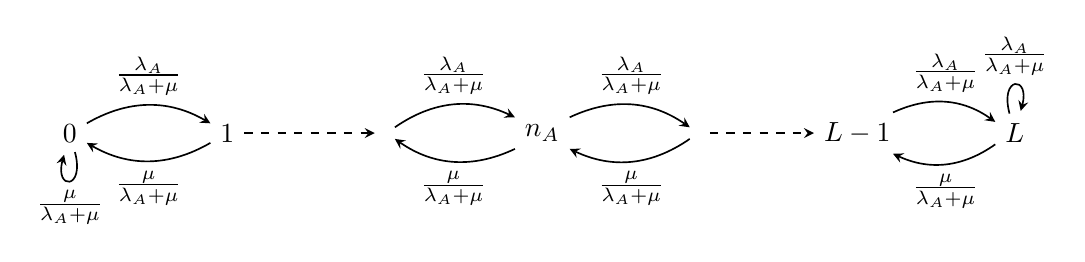
\begin{tikzpicture}[->, >=stealth, auto, semithick, node distance=2cm]
\tikzstyle{every state}=[fill=white,draw=black,text=black]

\node[] (A) {0};
\node[] (B) [right of=A] {1};
\node[] (C) [right of=B] {};
\node[] (D) [right of=C] {$\nA$};
\node[] (E) [right of=D] {};
\node[] (F) [right of=E] {$L-1$};
\node[] (G) [right of=F] {$L$};

\path (A) edge [loop below] node {$\frac{\rateS}{\rateA+\rateS}$} (A)
      (A) edge [bend left, above] node {$\frac{\rateA}{\rateA+\rateS}$} (B)
      (B) edge [bend left, below] node {$\frac{\rateS}{\rateA+\rateS}$} (A)
      (B) edge [dashed, above] node {} (C)
      (C) edge [bend left, above] node {$\frac{\rateA}{\rateA+\rateS}$} (D)
      (D) edge [bend left, below] node {$\frac{\rateS}{\rateA+\rateS}$} (C)
      (D) edge [bend left, above] node {$\frac{\rateA}{\rateA+\rateS}$} (E)
      (E) edge [bend left, below] node {$\frac{\rateS}{\rateA+\rateS}$} (D)
      (E)  edge [dashed, above] node {} (F)
      (F) edge [bend left, above] node {$\frac{\rateA}{\rateA+\rateS}$} (G)
      (G) edge [bend left, below] node {$\frac{\rateS}{\rateA+\rateS}$} (F)
      (G)  edge [loop above] node {$\frac{\rateA}{\rateA+\rateS}$} (G);

\end{tikzpicture}
\end{center}
\caption{Bounded Random-walk}
  \label{fig:ruin-4}
\end{figure} 


\begin{proof}
 Denoting by $\hittingt_{0}$ the hitting time of the state $0$,  we have  
\begin{equation}
\label{eq:U_n-A} 
\Utime_{\nA}=\Expect_{\nA}[\hittingt_{0}]\frac{1}{\rateA+\rateS}.
\end{equation}
For every $\statei$ in $\braces*{0,\dots,\naor}$, we define
\begin{equation}
\label{eq:h-i}
\exphit_{\statei} \coloneqq \Expect_{\statei}\bracks*{\hittingt_{0}}.
\end{equation}
Then, by \cref{Theo:hittingTime}, we have:
\begin{equation}
\label{eq:h-i-syst}  
\exphit_{\statei} = 
\begin{cases}
0 & \text{for $\statei=0$},\\
\displaystyle{1+\frac{\rateA}{\rateA+\rateS}\exphit_{\statei+1}+\frac{\rateS}{\rateA+\rateS}\exphit_{\statei-1}} & \text{for $0<\statei<L$},\\
\displaystyle{1+\frac{\rateA}{\rateA+\rateS}\exphit_{\naor}+\frac{\rateS}{\rateA+\rateS}\exphit_{\naor-1}} & \text{for $\statei=L$}.
\end{cases}
\end{equation}
As a consequence,
\begin{equation}
\label{eq:hna}
\exphit_{L}=\frac{\rateA+\rateS}{\rateS}+\exphit_{L-1}
\end{equation}
and, for every $0<\statei<L$,
\begin{equation}
\label{eq:h-i-h-i-1}
\begin{split}
\exphit_{\statei}-\exphit_{\statei-1} 
&=
\frac{\rateA+\rateS}{\rateS}+\frac{\rateA}{\rateS}(\exphit_{\statei+1}-\exphit_{\statei})\\
&=
\frac{\rateA+\rateS}{\rateS}\parens*{1+\frac{\rateA}{\rateS}}+\parens*{\frac{\rateA}{\rateS}}^2(\exphit_{\statei+2}-\exphit_{\statei+1})\\
&=
\frac{\rateA+\rateS}{\rateS}\sum_{\round=0}^{L-\statei-1}\parens*{\frac{\rateA}{\rateS}}^{\round} + \parens*{\frac{\rateA}{\rateS}}^{L-\statei}(\exphit_{L}-\exphit_{L-1})\\
&=
\frac{\rateA+\rateS}{\rateS}\sum_{\round=0}^{L-\statei}\parens*{\frac{\rateA}{\rateS}}^{\round}\\
&=
(1+\utilizationA)\sum_{\round=0}^{L-\statei}\utilizationA^{\round}.\\
\end{split}
\end{equation}
Then, for every $0<\statei<L$,
\begin{equation}
\label{eq:h-i-expr}
\begin{split}
\exphit_{\statei}
&=
 \exphit_{\statei-1}+ (1+\utilizationA)\sum_{\round=0}^{L-\statei}\utilizationA^{\round}=
 (1+\utilizationA)\sum_{j=0}^{i-1}\sum_{\round=0}^{L-(\statei-j)}\utilizationA^{\round}.\\
\end{split}
\end{equation}
Then, for every $0\leq \nA<L$, we have 
\begin{equation}
\label{eq:U-n-A}   
\Utime_{\nA}=\exphit_{\nA}/(\rateA+\rateS).
\end{equation}

\noindent Assume that $\utilizationA\neq 1$. If $0\leq \nA<L$, we have
\begin{equation}\label{eq:U_na}
\begin{split}
\Utime_{\nA}
&=
\frac{1}{\rateS}\sum_{j=0}^{\nA-1}\frac{1-\utilizationA^{L-\nA+j+1}}{1-\utilizationA}\\
&=
\frac{1}{\rateS-\rateA}\sum_{j=0}^{\nA-1}\parens*{1-\utilizationA^{L-\nA+j+1}}\\
&=
\frac{1}{\rateS-\rateA}\bracks*{\nA-\utilizationA^{L+1}\sum_{j=0}^{\nA-1}\utilizationA^{-(\nA-j)}}\\
&=
\frac{1}{\rateS-\rateA}\bracks*{\nA-\utilizationA^{L+1}\sum_{\round=1}^{\nA}\utilizationA^{-\round}}\\
&=
\frac{1}{\rateS-\rateA}\bracks*{\nA-\utilizationA^{L+1}\frac{\utilizationA^{-1}-\utilizationA^{-(\nA+1)}}{1-\utilizationA^{-1}}}\\
&=
\frac{1}{\rateS-\rateA}\bracks*{\nA-\frac{\utilizationA^{L+1}}{1-\utilizationA}\parens*{\utilizationA^{-\nA}-1}}\\
\end{split}
\end{equation}

If $\nA=L$, using \eqref{eq:hna}, \eqref{eq:U-n-A} and \eqref{eq:U_na} we have
\begin{equation}
\label{eq:U-naor}
\begin{split}    
\Utime_{L}
&=
\frac{1}{\rateS}+\frac{1}{\rateS-\rateA}\bracks*{L-1-\frac{\utilizationA^{L+1}}{1-\utilizationA}\parens*{\utilizationA^{-(L-1)}-1}}\\
&=
\frac{1}{\rateS-\rateA} \bracks*{L+\frac{\rateS-\rateA}{\rateS}-1-\frac{\utilizationA^{L+1}}{1-\utilizationA}\parens*{\utilizationA^{-(L-1)}-1}}\\
&=
\frac{1}{\rateS-\rateA} \bracks*{L-\utilizationA-\frac{\utilizationA^{L+1}}{1-\utilizationA}\parens*{\utilizationA^{-(L-1)}-1}}\\
&=
\frac{1}{\rateS-\rateA} \bracks*{L-\frac{\utilizationA^{L+1}}{1-\utilizationA}\parens*{\utilizationA^{-(L-1)}-1+(1-\utilizationA)\utilizationA^{-L}}}\\
&= 
\frac{1}{\rateS-\rateA} \bracks*{L-\frac{\utilizationA^{L+1}}{1-\utilizationA}\parens*{\utilizationA^{-L}-1}}.
\end{split}
\end{equation}
This concludes the proof for $\utilizationA\neq 1$.

Assume now that $\utilizationA=1$. If $0\leq\nA<L$, by \eqref{eq:h-i-expr} and \eqref{eq:U-n-A}.

\begin{equation}
    \label{eq:U-n-a-1}
\begin{split}
U_{\nA}
&=
\frac{1}{\rateS}\sum_{\round=0}^{\nA-1}(L-\nA+\round+1)\\
&=
\frac{1}{\rateS}\parens*{(L+1)\nA+\sum_{\round=0}^{\nA-1}(\round-\nA)}\\
&=
\frac{1}{\rateS}\parens*{(L+1)\nA-\sum_{\round=1}^{\nA}\round}\\
&=
\frac{1}{\rateS}\parens*{(L+1)\nA-\frac{\nA(\nA+1)}{2}}\\
&=
\frac{1}{2\rateS}\parens*{2(L+1)\nA-\nA(\nA+1)}\\
&=
\frac{\nA}{2\rateS}\parens*{2L+1-\nA}.
\end{split}
\end{equation}
If $\nA=L$,  using \eqref{eq:hna}, \eqref{eq:U-n-A} and \eqref{eq:U-n-a-1} we have
\begin{equation}
\begin{split}
U_{L}
&=
\frac{1}{\rateS}+\frac{L-1}{2\rateS}\parens*{L+2}\\
&=
\frac{2+\parens*{L-1}\parens*{L+2}}{2\rateS}\\
&=
\frac{L\parens*{L+1}}{2\rateS}.
\end{split}
\end{equation}
This conclude the proof for $\utilizationA=1$.
\end{proof}


\begin{proof}[Proof of \cref{le:E-time}]
    We begin noting that:
\begin{equation}
\label{eq:EtimePreempFS}
\begin{split}
\Htime(\nA,\nB)&=\Htime(\nA,\nB-1)+\Htime(0,1)\\
&=\Htime(\nA,0)+\nB\Htime(0,1)\\
&=\Utime_{\nA}+\nB\Htime(0,1).   
\end{split}
\end{equation}
Then, by  \cref{le:UtimeFullyStrat} we have 


\begin{equation}
\label{eq:UtimeFullStrat}
\Utime_{\nA} =\begin{cases} \frac{1}{\rateS(1-\utilizationA)}\bracks*{\nA-\frac{\utilizationA^{L+1}}{1-\utilizationA}\parens*{\utilizationA^{-\nA}-1}} & \text{ if } \utilizationA\neq 1,\\
\frac{\nA}{2\rateS}\parens*{2L+1-\nA} & \text{ if } \utilizationA=1.
\end{cases}
\end{equation}


To compute $\Htime(0,1)$ we need to consider two cases: either with probability $\rateS/(\rateS+\rateA)$ $\NB$ decreases by $1$,  or $\NA$ increases by $1$ with probability $\rateA/(\rateS+\rateA)$). 
Then,
\begin{equation}
\label{eq:E(0,1)}
\begin{split}    \Htime(0,1)&=\frac{\rateS}{\rateA+\rateS}\frac{1}{\rateS}+\frac{\rateA}{\rateS+\rateA}\Htime(1,1)\\
&=\frac{\rateS}{\rateA+\rateS}\frac{1}{\rateS}+\frac{\rateA}{\rateS+\rateA} \parens*{\Utime_1+\Htime(0,1)},
\end{split}
\end{equation}
from which we get 
\begin{align}
\Htime(0,1)\parens*{1-\frac{\rateA}{\rateS+\rateA}}
&=\frac{\rateS}{\rateA+\rateS}\frac{1}{\rateS}+\frac{\rateA}{\rateS+\rateA}\Utime_1 \\
\Htime(0,1)
&=\frac{1}{\rateS}+\utilizationA\Utime_1.
\end{align}
Hence, by \eqref{eq:UtimeFullStrat}, if $\utilizationA\neq 1$, we have

\begin{equation}\label{Eq:E-(0,0)-1}
\begin{split}
\Htime(0,1)& = \frac{1}{\rateS}+\frac{\utilizationA}{\rateS-\rateA} \parens*{1 - \frac{\utilizationA^{L+1}(\utilizationA^{-1}-1)}{1-\utilizationA}}\\
&=
\frac{1}{\rateS}+\frac{1}{\rateS-\rateA}\frac{\utilizationA}{1-\utilizationA} \parens*{1 -\utilizationA -\utilizationA^{L}+\utilizationA^{L+1}}\\
&=
\frac{1}{\rateS}+\frac{1}{\rateS-\rateA}\frac{\utilizationA}{1-\utilizationA} \parens*{1 -\utilizationA}\parens*{1-\utilizationA^{L}}\\
&=
\frac{\rateS-\rateA+\rateA\parens*{1-\utilizationA^{L}}}{\rateS(\rateS-\rateA)}\\
&=
\frac{1-\utilizationA^{L+1}}{\rateS-\rateA}
\end{split}
\end{equation}
Plugging \eqref{Eq:E-(0,0)-1} and \eqref{eq:UtimeFullStrat} into \eqref{eq:EtimePreempFS}, for $\utilizationA\neq 1$ we obtain
\begin{equation*}
\Htime(\nA,\nB)= \frac{1}{(\rateS-\rateA)} \bracks*{\nB\parens*{1 - \utilizationA^{L+1}}+  \nA-\frac{\utilizationA^{L+1}}{1-\utilizationA} \parens*{\utilizationA^{-\nA}-1}}.    
\end{equation*}

If $\utilizationA=1$ we have
\begin{equation}\label{eq:E-(0,0)-2}
\Htime(0,1)=\frac{1+L}{\rateS},
\end{equation}
and
\begin{equation}
    \Htime(\nA,\nB)=\frac{1}{2\rateS}\bracks*{\nA(2L+1-\nA)+2\nB(1+L)}.
\end{equation}

\end{proof}





\begin{proof}[Proof of \cref{cl:G-increasing}]
We show that $G'(\nAB)\geq 0$ for $\Veq\leq \nAB \leq \Teq-1$.
\begin{align}
G'(\nAB)=&\frac{1}{\rateS(1-\utilizationA)}\cdot\frac{\parens*{1-\utilizationA^{\naor+1}+(\naor+1)\utilizationA^{\Teq-\nAB}\ln{\utilizationA}}\parens*{1-\utilizationA^{\Teq-\nAB}}}{\parens*{1-\utilizationA^{\Teq-\nAB}}^2}\nonumber\\
&- \frac{1}{\rateS(1-\utilizationA)}\cdot\frac{\utilizationA^{\Teq-\nAB}\ln{\utilizationA}\parens*{(\nAB+1-\Veq)\parens*{1-\utilizationA^{\naor+1}}-(\naor+1)\parens*{\utilizationA^{\Teq-\nAB}-\utilizationA^{\naor+1}}}}{\parens*{1-\utilizationA^{\Teq-\nAB}}^2}\nonumber\\
=&\frac{\parens*{1-\utilizationA^{\naor+1}}\parens*{1-\utilizationA^{\Teq-\nAB}}+(\naor+1)\utilizationA^{\Teq-\nAB}\ln{\utilizationA}}{\rateS(1-\utilizationA)\parens*{1-\utilizationA^{\Teq-\nAB}}^2}\nonumber\\
&-\frac{\utilizationA^{\Teq-\nAB}\ln{\utilizationA}\parens*{(\nAB+1-\Veq)\parens*{1-\utilizationA^{\naor+1}}+(\naor+1)\utilizationA^{\naor+1}}}{\rateS(1-\utilizationA)\parens*{1-\utilizationA^{\Teq-\nAB}}^2}\nonumber\\
=&\frac{\parens*{1-\utilizationA^{\naor+1}}\bracks*{\parens*{1-\utilizationA^{\Teq-\nAB}}+(\naor+1)\utilizationA^{\Teq-\nAB}\ln{\utilizationA}-\utilizationA^{\Teq-\nAB}\ln{\utilizationA}(\nAB+1-\Veq)}}{\rateS(1-\utilizationA)\parens*{1-\utilizationA^{\Teq-\nAB}}^2}\nonumber\\
=&\frac{1-\utilizationA^{\naor+1}}{\rateS(1-\utilizationA)}\cdot\frac{1-\utilizationA^{\Teq-\nAB}+(\Teq-\nAB)\utilizationA^{\Teq-\nAB}\ln{\utilizationA}}{\parens*{1-\utilizationA^{\Teq-\nAB}}^2}\nonumber\\
=&\frac{1-\utilizationA^{\naor+1}}{\rateS(1-\utilizationA)}\cdot\frac{1-\utilizationA^{\Teq-\nAB}\parens*{1-\ln{\utilizationA^{\Teq-\nAB}}}}{\parens*{1-\utilizationA^{\Teq-\nAB}}^2}.\nonumber
\end{align}
Now, with the change of variable $x=\utilizationA^{\Teq-\nAB}$, the result follows from the following inequality:
\begin{equation*}
\label{eq:inequality-x} 
1-x(1-\ln{x}) \geq 0,\quad\text{for } x>0.
\qedhere
\end{equation*}  
\end{proof}



\section*{Acknowledgments}
\label{se:acknowledments}

\subsection*{Funding}
 
Maurizio D'Andrea and Marco Scarsini are members of GNAMPA-INdAM.
Their work was partially supported by the  MIUR PRIN 2022EKNE5K ``Learning in markets and society.'' 

\bibliographystyle{apalike}
\bibliography{bib-multiclass-queues}







\end{document}

